\documentclass[slidestop,mathserif,compress,xcolor=svgnames]{beamer} 
\mode<presentation>
{  
  \setbeamertemplate{background canvas}[vertical shading][bottom=blue!5,top=blue!5]
  \setbeamertemplate{navigation symbols}{}%{\insertsectionnavigationsymbol}
  \usetheme{LSU}
%  default infolines miniframes shadow sidebar smoothbars smoothtree split tree
%    \useoutertheme{shadow}
}

\usepackage{pgf,pgfarrows,pgfnodes,pgfautomata,pgfheaps,pgfshade}
\usepackage{amsmath,amssymb,amsfonts,subfigure}
\usepackage{multirow,rotating}
\usepackage{tabularx}
\usepackage{booktabs}
\usepackage{colortbl}
\usepackage{tikz}
\usefonttheme{serif}
\usetikzlibrary{shapes,arrows}
\usetikzlibrary{calc}
\pgfdeclarelayer{background}
\pgfdeclarelayer{foreground}
\pgfsetlayers{background,main,foreground}
\usepackage[latin1]{inputenc}
\usepackage{colortbl}
\usepackage[english]{babel}
\usepackage{hyperref}
\usepackage[normalem]{ulem}
% \usepackage{movie15}
\hypersetup{
  pdftitle={Advanced Concepts in Fortran 90},
  pdfauthor={Alexander B. Pacheco, User Services Consultant, Louisiana State University}
}
%\usepackage{movie15}
\usepackage{times}

\setbeamercovered{dynamic}
\beamersetaveragebackground{DarkBlue!2}
\beamertemplateballitem

\usepackage[english]{babel}
\usepackage[latin1]{inputenc}
\usepackage{times}
\usepackage{amsmath}
\usepackage[T1]{fontenc}
\usepackage{graphicx}
\definecolor{DarkGreen}{rgb}{0.0,0.3,0.0}
\definecolor{darkgreen}{rgb}{0.0,0.6,0.0}
\definecolor{Blue}{rgb}{0.0,0.0,0.8} 
\definecolor{dodgerblue}{rgb}{0.1,0.1,1.0}
\definecolor{indigo}{rgb}{0.41,0.1,0.0}
\definecolor{seagreen}{rgb}{0.1,1.0,0.1}
\DeclareSymbolFont{extraup}{U}{zavm}{m}{n}
\DeclareMathSymbol{\vardiamond}{\mathalpha}{extraup}{87}
\newcommand*\up{\textcolor{green}{%
  \ensuremath{\blacktriangle}}}
\newcommand*\down{\textcolor{red}{%
  \ensuremath{\blacktriangledown}}}
\newcommand*\const{\textcolor{darkgray}%
  {\textbf{--}}}
\newcommand{\bftt}[1]{\textbf{\texttt{#1}}}

\setbeamercolor{uppercol}{fg=white,bg=red!30!black}%
\setbeamercolor{lowercol}{fg=black,bg=red!15!white}%
\setbeamercolor{uppercol1}{fg=white,bg=blue!30!black}%
\setbeamercolor{lowercol1}{fg=black,bg=blue!15!white}%%
\setbeamercolor{uppercol2}{fg=white,bg=green!30!black}%
\setbeamercolor{lowercol2}{fg=black,bg=green!15!white}%
\setbeamercolor{uppercol3}{fg=white,bg=green!50!red!50!black}%
\setbeamercolor{lowercol3}{fg=black,bg=green!60!red!30!white}%
\setbeamercolor{uppercol4}{fg=white,bg=green!30!blue!50!black}%
\setbeamercolor{lowercol4}{fg=black,bg=green!30!blue!50!white}%
\newenvironment{colorblock}[4]
{
\setbeamercolor{upperblock}{fg=#1,bg=#2}
\setbeamercolor{lowerblock}{fg=#3,bg=#4}
\begin{beamerboxesrounded}[upper=upperblock,lower=lowerblock,shadow=true]}
{\end{beamerboxesrounded}}
\newenvironment{ablock}[0]
{
\begin{beamerboxesrounded}[upper=uppercol,lower=lowercol,shadow=true]}
{\end{beamerboxesrounded}}
\newenvironment{bblock}[0]
{
\begin{beamerboxesrounded}[upper=uppercol1,lower=lowercol1,shadow=true]}
{\end{beamerboxesrounded}}
\newenvironment{eblock}[0]
{
\begin{beamerboxesrounded}[upper=uppercol2,lower=lowercol2,shadow=true]}
{\end{beamerboxesrounded}}
\newenvironment{beblock}[0]
{
\begin{beamerboxesrounded}[upper=uppercol3,lower=lowercol3,shadow=true]}
{\end{beamerboxesrounded}}
\newenvironment{eeblock}[0]
{
\begin{beamerboxesrounded}[upper=uppercol4,lower=lowercol4,shadow=true]}
{\end{beamerboxesrounded}}

% Fix font size of nested itemize/enumerate
\setbeamerfont{itemize/enumerate body}{}
\setbeamerfont{itemize/enumerate subbody}{size=\scriptsize}
\setbeamerfont{itemize/enumerate subsubbody}{size=\scriptsize}

\title[Advanced Concepts F90]{Advanced Concepts in Fortran 90}


\author[Alex Pacheco]{\large{Alexander~B.~Pacheco}}
       
\institute[HPC@LSU - http://www.hpc.lsu.edu] {\inst{}\footnotesize{User Services Consultant\\LSU HPC \& LONI\\sys-help@loni.org}}

\date[{Feb 13-16, 2012\hspace{2cm}}]{\scriptsize{LONI Workshop: Fortran Programming\\Louisiana State University\\Baton Rouge\\Feb 13-16, 2012}}
     
\subject{Talks}
% This is only inserted into the PDF information catalog. Can be left
% out. 




% If you have a file called "university-logo-filename.xxx", where xxx
% is a graphic format that can be processed by latex or pdflatex,
% resp., then you can add a logo as follows:

% Main Logo on bottom left
\pgfdeclareimage[height=0.55cm]{its-logo}{LONI}
\logo{\pgfuseimage{its-logo}}
% University Logo on top left
\pgfdeclareimage[height=0.55cm]{university-logo}{LSUGeauxPurp}
\tllogo{\pgfuseimage{university-logo}}
% Logo at top right
\pgfdeclareimage[height=0.6cm]{institute-logo}{PUR_BLK_HOR}
\trlogo{\pgfuseimage{institute-logo}}
% Logo at bottom right
\pgfdeclareimage[height=0.55cm]{hpc-logo}{CCT}
\brlogo{\pgfuseimage{hpc-logo}}


% Delete this, if you do not want the table of contents to pop up at
% the beginning of each subsection:
  \AtBeginSection[]
  {
    \begin{frame}<beamer>
     \frametitle{\small{Outline}}
      \small
      \tableofcontents[currentsection,currentsubsection]
    \end{frame}
  }

\begin{document}
\scriptsize

\frame{\titlepage}

\begin{frame}[label=toc,squeeze]
  \footnotesize
  \frametitle{\small{Outline}}
  \tableofcontents
\end{frame}


%\part{Introduction}
\section{Review}
\begin{frame}[allowframebreaks]
  \frametitle{\small Review}
  \begin{block}{\scriptsize Logical Structure}
    \begin{enumerate}
      \item program name
      \item declaration of variable types
      \item read input
      \item do calculations
      \item write output
      \item end program
    \end{enumerate}
  \end{block}

  \begin{columns}
    \column{6cm}
    \begin{bblock}{Example Code}
      \begin{tabbing}
        \textbf{\texttt{pro}}\=\textbf{\texttt{gram}} \texttt{hello} \\
        \> \textbf{\texttt{implicit none}} \\
        \> \textbf{\texttt{character(len=100) ::}} \texttt{your\_name} \\
        \\
        \> \texttt{print *, 'Your name please'} \\
        \> \texttt{read *, your\_name} \\
        \> \texttt{print *, 'Hello ', your\_name} \\
        \\
        \textbf{\texttt{end program}} \texttt{hello}
      \end{tabbing}
    \end{bblock}
    \column{4cm}
    \begin{beblock}{Output}
      \begin{tabbing}
        \%>ifort -o hello hello.f90 \\
        \%>\=./hello \\
        \>{\color{red}Your Name Please} \\
        \>{\color{black}``Alex Pacheco''} \\
        \>{\color{red}Hello Alex Pacheco} \\
        \%>
      \end{tabbing}
    \end{beblock}
  \end{columns}

  \begin{block}{\scriptsize Fortran Free Source Form}
    \begin{itemize}
      \item Fortran 90/95/2003: free form source, a line can contain up to 132 characters
      \item Inline comments initiated by !
      \item Statements are continued by appending \& 
      \item program name and variables: up to 31 letters, digits and underscores ( \_ )
      \item {\color{red}names must begin with a letter}; digits and underscores are not allowed
      \item multiple commands on single line separated by semi-colon ( ; )
    \end{itemize}
  \end{block}

  \begin{ablock}{Coding Style}
    \begin{itemize}
      \item always use \textbf{\texttt{implicit none}}
      \item avoid using mixed cases i.e. upper and lower case
      \item[] Some coders prefer fortran keywords, intrinsic functions and user defined entities as upper case while rest of the code in lower case. I prefer everything in lower case!
      \item[] For visibility, all intrinsic functions and user defined entities are in bold except when displaying a code available from the exercise directories
      \item Remember someone else will continue the development of your code, so
      \item[] INDENT your code, it makes it easier to read
      \item[] Add meaningfull comments where ever possible
    \end{itemize}
  \end{ablock}

 % \begin{bblock}{Significance of Blanks}
 %   \begin{itemize}
 %     \item Blanks must not appear within
 %     \begin{enumerate}
 %       \item keywords
 %       {\tiny
 %       \item[] \textbf{\texttt{integer :: nstep}}  ! valid keyword
 %       \item[] \textbf{\texttt{int eger :: nstep}} ! not a valid keyword
 %       }
 %       \item names
 %       {\tiny
 %       \item[] \textbf{\texttt{real :: force\_t}}   ! valid name
 %       \item[] \textbf{\texttt{real :: force t}}   ! not a valid name
 %       }
 %     \end{enumerate}
 %     \item Blanks must appear
 %     \begin{enumerate}
 %       \item between two separate keywords
 %       \item between keywords and names not separated by punctuation or special characters
 %       {\tiny
 %       \item[] \textbf{\texttt{integer function fit(i)}} ! valid
 %       \item[] \textbf{\texttt{integerfunction fit(i)}} ! not valid
 %       \item[] \textbf{\texttt{integer functionfit(i)}} ! not valid
 %       }
 %     \end{enumerate}
 %   \end{itemize}
 % \end{bblock}
  \framebreak
  \begin{block}{\scriptsize Declarations and Attributes}
    \begin{itemize}
      \item Can state \textbf{\texttt{implicit none}}: all variables must be declared
      \item[$\vardiamond$] Syntax:
      \item[] \textbf{\texttt{<type> [,<attribute-list>] [::]}} \texttt{<variable-list> [=<value>]}
      \item[] \textbf{\texttt{<type>}} : data types i.e. integer, real, complex, character or logical
      \item[] \textbf{\texttt{attributes}} : dimension, parameter, pointer, target, allocatable, optional, intent
    \end{itemize}
  \end{block}
  \begin{bblock}{Examples of valid declarations}
    \begin{tabbing}
      \textbf{\texttt{sub}}\=\textbf{\texttt{routine}} \texttt{aroutine(x,i,j)} \\
      \>\textbf{\texttt{implicit none}} \\
      \>\textbf{\texttt{real, intent(in) ::}} \texttt{x} \\
      \>\textbf{\texttt{logical ::}} \texttt{what} \\
      \>\textbf{\texttt{real,dimension(10,10) ::}} \texttt{y, z(10)} \\
      \>\textbf{\texttt{character(len=*),parameter ::}} \texttt{somename} \\
      \>\textbf{\texttt{integer, intent(out) ::}} \texttt{i,j} \\
      \> $\cdots$ \\
      \textbf{\texttt{end subroutine}} \texttt{aroutine}
    \end{tabbing}
  \end{bblock}
  \framebreak
  \begin{columns}
    \column{6cm}
    \begin{block}{\scriptsize Data Types}
      \begin{description}
      \item[INTEGER:]exact whole numbers
      \item[REAL:]real, fractional numbers
      \item[COMPLEX:]complex, fractional numbers
      \item[LOGICAL:]boolean values
      \item[CHARACTER:]strings
      \end{description}
    \end{block}
    \column{2.8cm}
    \begin{block}{\scriptsize Arithmetic Operators}
      \begin{itemize}
      \item[+]: addition
      \item[-]: subtraction
      \item[*]: multiplication
      \item[/]: division
      \item[**]: exponentiation
      \end{itemize}
    \end{block}
  \end{columns}
%  \framebreak
  \begin{columns}
    \column{4cm}
    \begin{block}{\scriptsize Relational Operators}
      \begin{itemize}
        \item[==]: equal to
        \item[/=]: not equal to
        \item[<]: less than
        \item[<=]: less than or equal to
        \item[>]: greater than
        \item[>=]: greater than or equal to
      \end{itemize}
    \end{block}
    \column{3cm}
    \begin{block}{\scriptsize Logical Expressions}
      \begin{description}
        \item[.TRUE.]  
        \item[.FALSE.]
        \item[.AND.]
        \item[.OR.]
        \item[.NOT.] 
      \end{description}
    \end{block}
  \end{columns}
  \begin{block}{{\scriptsize Operator Precedence}}
    \begin{center}
      {\tiny
      \begin{tabular}{ccc}
        Operator & Precedence & Example \\
        \hline
        expression in () & Highest & (a+b) \\
        user-defined monadic & - & .inverse.a \\
        ** & - & 10**4 \\
        * or / & - & 10*20 \\
        monadic + or - & - & -5 \\
        dyadic + or - & - & 1+5 \\
        // & - & str1//str2 \\
        relational operators & - & a > b \\
        .not. & - & .not.allocated(a) \\
        .and. & - & a.and.b \\
        .or. & - & a.or.b \\
        .eqv. or .neqv. & - & a.eqv.b \\
        user defined dyadic & Lowest & x.dot.y\\
        \hline
      \end{tabular}
      }
    \end{center}
  \end{block}
  \begin{block}{}
    {\tiny
    \begin{itemize}
      \item x = a + b/5.0 - c**2 + 2.0*e
      \item[] exponentiation (**) has highest precedence followed by / and *
      \item The above expression is equivalent to
      \item x = a + b/5.0 - c' + 2.0*e = a + b' - c' + 2.0*e = a + b' - c' + e'
      \item[] where b' = b/5.0 , c' = c**2 and e' = 2.0*e
      \item x = a + b/5.0 - c**2 + (2.0*e)
      \item equivalent to x = a + b/5.0 - c**2 + e' = a + b/5.0 - c' + e' = a + b' - c' + e'
    \end{itemize}
    }
  \end{block}
\end{frame}

\begin{frame}
  \frametitle{\small Guidelines for Slides}
  \begin{columns}
    \column{5cm}
    \begin{block}{\scriptsize Code in this block}
      Generic Code explaining Fortran Programming Structure or Style
    \end{block}
    \column{5cm}
    \begin{eblock}{Code in this block}
      Code in Exercises directory\\
      /work/apacheco/F90-workshop/Exercises
    \end{eblock}
  \end{columns}
  \vspace{1cm}
  \begin{columns}
    \column{5cm}
    \begin{bblock}{Code in this block}
      Code written only to explain content on current or previous slide
    \end{bblock}
    \column{5cm}
    \begin{eeblock}{Code in this block}
      Code from Exercises directory but modified to describe content on current or previous slide
    \end{eeblock}
  \end{columns}
  \vspace{1cm}
  \begin{columns}
    \column{5cm}
    \begin{beblock}{}
      Output from code
    \end{beblock}
  \end{columns}
\end{frame}

\section{Intrinsic Functions}
\begin{frame}[t]
  \frametitle{\small Intrinsic Functions}
  \begin{itemize}
    \item Fortran provides a set of intrinsic functions
  \end{itemize}
  \begin{columns}
    \column{6cm}
    {\tiny
      \begin{block}{\scriptsize Arithmetic Functions}
        \begin{center}
          \begin{tabular}{ccc}
            Function & Action & Example \\
            \hline
            INT & conversion to integer & J=INT(X) \\
            REAL & conversion to real & X=REAL(J) \\
            CMPLX & conversion to complex & A=CMPLX(X,Y) \\
            ABS & absolute value & Y=ABS(X) \\
            MOD & remainder when I divided by J & K=MOD(I,J) \\
            SQRT & square root & Y=SQRT(X) \\
            EXP & exponentiation & Y=EXP(X) \\
            LOG & natural logarithm & Y=LOG(X) \\
            LOG10 & logarithm to base 10 & Y=LOG10(X) \\
            \hline
          \end{tabular}
        \end{center}
      \end{block}
    }
    \column{5cm}
    {\tiny
      \begin{block}{\scriptsize Trignometric Functions}
        \begin{center}
          \begin{tabular}{ccc}
            Function & Action & Example \\
            \hline
            SIN & sine & X=SIN(Y) \\
            COS & cosine & X=COS(Y) \\
            TAN & tangent & X=TAN(Y) \\
            ASIN & arcsine & X=ASIN(Y) \\
            ACOS & arccosine & X=ACOS(Y) \\
            ATAN & arctangent & X=ATAN(Y) \\
            ATAN2 & arctangent(a/b) & X=ATAN2(A,B) \\
            \hline
          \end{tabular}
        \end{center}
      \end{block}
    }
  \end{columns}
\end{frame}


\begin{frame}[fragile,allowframebreaks]
  \frametitle{\small KIND Parameter}
  \begin{block}{}
    \begin{itemize}
      \item \textbf{kind} parameters provide a way to parameterize the selection of different possible machine representations for each intrinsic data types.
      \item The \textbf{kind} parameter is an integer which is processor dependent.
      \item There are only 2(3) kinds of reals: 4-byte, 8-byte (and 16-byte), respectively known as single, double (and quadruple) precision.
      \item The corresponding \textbf{kind} numbers are 4, 8 and 16 (most compilers)
      \item The value of the \textbf{kind} parameter is usually not the number of decimal digits of precision or range; on many systems, it is the number of bytes used to represent the value.
      \item The intrinsic functions \textbf{selected\_int\_kind} and \textbf{selected\_real\_kind} may be used to select an appropriate \textbf{kind} for a variable or named constant.
    \end{itemize}
  \end{block}
  {\fontsize{4}{5}
    \begin{eblock}{}
      \begin{verbatim}
program kind_function

  implicit none
  integer,parameter :: dp = selected_real_kind(15) 
  integer,parameter :: ip = selected_int_kind(15) 
  integer(kind=4) :: i
  integer(kind=8) :: j
  integer(ip) :: k
  real(kind=4) :: a
  real(kind=8) :: b
  real(dp) :: c

  print '(a,i2,a,i4)', 'Kind of i = ',kind(i), '  with range =', range(i)
  print '(a,i2,a,i4)', 'Kind of j = ',kind(j), '  with range =', range(j)
  print '(a,i2,a,i4)', 'Kind of k = ',kind(k), '  with range =', range(k)
  print '(a,i2,a,i2,a,i4)', 'Kind of real a = ',kind(a),&
       '  with precision = ', precision(a),&
       '  and range =', range(a)
  print '(a,i2,a,i2,a,i4)', 'Kind of real b = ',kind(b),&
       '  with precision = ', precision(b),&
       '  and range =', range(b)
  print '(a,i2,a,i2,a,i4)', 'Kind of real c = ',kind(c),&
       '  with precision = ', precision(c),&
       '  and range =', range(c)

end program kind_function
      \end{verbatim}
    \end{eblock}
    \begin{beblock}{}
        \begin{verbatim}
[apacheco@qb4 examples] ./kindfns 
Kind of i =  4  with range =   9
Kind of j =  8  with range =  18
Kind of k =  8  with range =  18
Kind of real a =  4  with precision =  6  and range =  37
Kind of real b =  8  with precision = 15  and range = 307
Kind of real c =  8  with precision = 15  and range = 307
        \end{verbatim}
    \end{beblock}
  }
\end{frame}

\section{Control Constructs}
\begin{frame}
  \frametitle{\small Control Constructs}
  \begin{block}{}
    \begin{itemize}
      \item A Fortran program is executed sequentially
      \begin{tabbing}
        pr\=ogram somename \\
        \> variable declarations \\
        \> statement 1 \\
        \> statement 2 \\
        \> $\cdots$ \\
        end program somename
      \end{tabbing}
      \item Control Constructs change the sequential execution order of the program
      \begin{enumerate} \itemsep1pt \parskip0pt \parsep0pt
        \item Conditionals: IF
        \item Loops: DO
        \item Switches: SELECT/CASE
        \item Branches: GOTO (obsolete in Fortran 95/2003, use CASE instead)
      \end{enumerate}
    \end{itemize}
  \end{block}
\end{frame}

\subsection{Conditionals}

\begin{frame}
  \frametitle{\small If Statement}
  \begin{block}{\scriptsize The general form of the \textbf{\texttt{if}} statement}
  \textbf{\texttt{if}} (\textit{logical expression}) \textit{statement}
  \end{block}
  \begin{itemize}
    \item When the \textbf{\texttt{if}} statement is executed, the logical expression is evaluated. 
    \item If the result is true, the statement following the logical expression is executed; otherwise, it is not executed.
    \item The statement following the logical expression \textbf{cannot} be another \textbf{\texttt{if}} statement. Use the \textbf{\texttt{if-then-else}} construct instead.
  \end{itemize}
  \begin{columns}
    \column{5cm}
    \begin{bblock}{}
      \textbf{\texttt{if}} \texttt{(value < 0 ) value = 0}
    \end{bblock}
  \end{columns}
\end{frame}

\begin{frame}[allowframebreaks]
  \frametitle{\small If-then-else Construct}
  \begin{itemize}
    \item The \textbf{\texttt{if-then-else}} construct permits the selection of one of a number of blocks during execution of a program
    \item The \textbf{if-then} statement is executed by evaluating the logical expression.
    \item If it is true, the block of statements following it are executed. Execution of this block completes the execution of the entire \textbf{if} construct.
    \item If the logical expression is false, the next matching \textbf{else if}, \textbf{else} or \textbf{end if} statement following the block is executed.
  \end{itemize}
  
  \begin{columns}
    \column{5cm}
    \begin{block}{ }
      \begin{tabbing}
        \textbf{\texttt{if}} \=(\textit{logical expression}) \textbf{\texttt{then}} \\
        \> \textit{block of statements} \\
        \textbf{\texttt{else if}} (\textit{logical expression}) \textbf{\texttt{then}} \\
        \> \textit{block of statements} \\
        \textbf{\texttt{else if} $\cdots$} \\
        \> $\vdots$ \\
        \textbf{\texttt{else}} \\
        \> \textit{block of statements} \\
        \textbf{\texttt{end if}}
      \end{tabbing}
    \end{block}
  \end{columns}
  
  \framebreak
  \begin{itemize}
    \item Examples:
  \end{itemize}
  \begin{columns}
    \column{4cm}
    \begin{bblock}{Letter Grade}
      {\tiny
      \begin{tabbing}
        \textbf{\texttt{if}} \=\texttt{(x < 50 )} \textbf{\texttt{then}} \\
        \> \texttt{GRADE = 'F'} \\
        \textbf{\texttt{else if}} \texttt{(x < 60 )} \textbf{\texttt{then}} \\
        \> \texttt{GRADE = 'D'} \\
        \textbf{\texttt{else if}} \texttt{(x < 70 )} \textbf{\texttt{then}} \\
        \> \texttt{GRADE = 'C'} \\
        \textbf{\texttt{else if}} \texttt{(x < 80 )} \textbf{\texttt{then}} \\
        \> \texttt{GRADE = 'B'} \\
        \textbf{\texttt{else}} \\
        \> \texttt{GRADE = 'A'} \\
        \textbf{\texttt{end if}}
      \end{tabbing}
      }
    \end{bblock}
    \column{6cm}
    \begin{bblock}{Find minimum of a,b and c}
      {\tiny
      \begin{tabbing}
        \textbf{\texttt{if}} \=\texttt{(a < b .and. a < c)} \textbf{\texttt{then}} \\
        \> \texttt{result = a} \\
        \textbf{\texttt{else if}} \texttt{(b < a  .and. b < c )} \textbf{\texttt{then}}\\
        \> \texttt{result = b} \\
        \textbf{\texttt{else}} \\
        \> \texttt{result = c} \\
        \textbf{\texttt{end if}}
      \end{tabbing}
      }
    \end{bblock}
  \end{columns}
  
  \framebreak
  \begin{itemize}
    \item The \textbf{else if} and \textbf{else} statements and blocks may be omitted.
    \item If \textbf{else} is missing and none of the logical expressions are true, the \textbf{if-then-else} construct has no effect.
    \item The \textbf{end if} statement must not be omitted.
    \item The \textbf{if-then-else} construct can be nested and named.
  \end{itemize}
  \begin{columns}
    \column{6cm}
    \begin{block}{\scriptsize no \bftt{else if}}
      \begin{tabbing}
        [co\=nstruct name:] \textbf{\texttt{if}} (\textit{logical expression}) \textbf{\texttt{then}} \\
        \> \textit{block of statements} \\
        \textbf{\texttt{else}} \\
        \> \textit{block of statements} \\
        \>[na\=me:] \textbf{\texttt{if}} (\textit{logical expression}) \textbf{\texttt{then}} \\
        \>\>\textit{block of statements} \\
        \>\textbf{\texttt{end if}} [name] \\
        \textbf{\texttt{end if}} [construct name]
      \end{tabbing}
    \end{block}
    \column{5cm}
    \begin{block}{\scriptsize no \bftt{else}}
      \begin{tabbing}
        \textbf{\texttt{if}} \=(\textit{logical expression}) \textbf{\texttt{then}} \\
        \> \textit{block of statements} \\
        \textbf{\texttt{else if}} (\textit{logical expression}) \textbf{\texttt{then}} \\
        \> \textit{block of statements} \\
        \textbf{\texttt{else if}} (\textit{logical expression}) \textbf{\texttt{then}} \\
        \> \textit{block of statements} \\
        \textbf{\texttt{end if}}
      \end{tabbing}
    \end{block}
  \end{columns}
\end{frame}

\begin{frame}[fragile,allowframebreaks]
  \frametitle{\small Finding roots of quadratic equation}
  {\fontsize{4}{5}
    \begin{eblock}{}
      \begin{verbatim}
program roots_of_quad_eqn

  implicit none

  real(kind=8) :: a,b,c
  real(kind=8) :: roots(2),d

  print *, '============================================'
  print *, ' Program to solve a quadratic equation'
  print *, '    ax^2 + bx + c = 0 '
  print *, ' If d = b^2 - 4ac >= 0 '
  print *, '   then solutions are: '
  print *, '     (-b +/- sqrt(d) )/2a '
  print *, '============================================'

  ! read in coefficients a, b, and c
  write(*,*) 'Enter coefficients a,b and c'
  read(*,*) a,b,c
  write(*,*)
  write(*,*) ' Quadratic equation to solve is: '
  write(*,fmt='(a,f5.3,a,f5.3,a,f5.3,a)') '   ',a,'x^2 + ',b,'x + ',c,' = 0'
  write(*,*)

  outer: if ( a == 0d0 ) then
     middle: if ( b == 0.d0 ) then
        inner: if ( c == 0.d0 ) then
           write(*,*) 'Input equation is 0 = 0'
        else
           write(*,*) 'Equation is unsolvable'
           write(*,fmt='(a,f5.3,a)') ' ',c,' = 0'
        end if inner
     else
        write(*,*) 'Input equation is a Linear equation with '
        write(*,fmt='(a,f6.3)') ' Solution: ', -c/b
     end if middle
  else
     d = b*b - 4d0*a*c
     dis0: if ( d > 0d0 ) then
      \end{verbatim}
    \end{eblock}
    \framebreak
    \begin{eblock}{}
      \begin{verbatim}
        d = sqrt(d)
        roots(1) = -( b + d)/(2d0*a) ; roots(2) = -( b - d)/(2d0*a)
        write(*,fmt='(a,2f12.6)') 'Solution: ', roots(1),roots(2)
     else if ( d == 0.d0 ) then
        write(*,fmt='(a,f12.6)') 'Both solutions are equal: ', -b/(2d0*a)
     else
        write(*,*) 'Solution is not real'
        d = sqrt(abs(d))
        roots(1) = d/(2d0*a)
        roots(2) = -d/(2d0*a)
        write(*,fmt='(a,ss,f6.3,sp,f6.3,a2,a,ss,f6.3,sp,f6.3,a2)') &
             ' (',-b/(2d0*a),sign(roots(1),roots(1)),'i)',' and (',-b/(2d0*a),sign(roots(2),roots(2)),'i)'
     end if dis0
  end if outer
end program roots_of_quad_eqn
      \end{verbatim}
    \end{eblock}
    \begin{columns}
      \column{3.7cm}
      \begin{beblock}{}
        \begin{verbatim}
[apacheco@qb4 examples] ./root.x 
 ============================================
  Program to solve a quadratic equation
     ax^2 + bx + c = 0 
  If d = b^2 - 4ac >= 0 
    then solutions are: 
      (-b +/- sqrt(d) )/2a 
 ============================================
 Enter coefficients a,b and c
1 2 1

  Quadratic equation to solve is: 
   1.000x^2 + 2.000x + 1.000 = 0

Both solutions are equal:    -1.000000
        \end{verbatim}
      \end{beblock}
      \column{3.7cm}
      \begin{beblock}{}
        \begin{verbatim}
[apacheco@qb4 examples] ./root.x 
 ============================================
  Program to solve a quadratic equation
     ax^2 + bx + c = 0 
  If d = b^2 - 4ac >= 0 
    then solutions are: 
      (-b +/- sqrt(d) )/2a 
 ============================================
 Enter coefficients a,b and c
0 1 2

  Quadratic equation to solve is: 
   0.000x^2 + 1.000x + 2.000 = 0

 Input equation is a Linear equation with 
 Solution: -2.000
        \end{verbatim}
      \end{beblock}
      \column{3.7cm}
      \begin{beblock}{}
        \begin{verbatim}
[apacheco@qb4 examples] ./root.x 
 ============================================
  Program to solve a quadratic equation
     ax^2 + bx + c = 0 
  If d = b^2 - 4ac >= 0 
    then solutions are: 
      (-b +/- sqrt(d) )/2a 
 ============================================
 Enter coefficients a,b and c
2 1 1

  Quadratic equation to solve is: 
    2.000x^2 +  1.000x +  1.000 = 0

 Solution is not real
 (-0.250+0.661i) and (-0.250-0.661i)
        \end{verbatim}
      \end{beblock}
    \end{columns}
  }
\end{frame}

\subsection{Switches}
\begin{frame}[fragile,allowframebreaks]
  \frametitle{\small Case Construct}
  \begin{itemize}
    \item The \textbf{case} construct permits selection of one of a number of different block of instructions.
    \item The value of the expression in the \textbf{select case} should be an integer or a character string.
  \begin{columns}
    \column{5cm}
    \begin{block}{}
      \begin{tabbing}
        [co\=nstruct name:] \textbf{select case} (\textit{expression})\\
        \> \textbf{ca}\=\textbf{se} (\textit{case selector})\\
        \> \> \texttt{block of statements}\\
        \> \textbf{case} (\textit{case selector})\\
        \> \> \texttt{block of statements}\\
        \> \> $\vdots$ \\
        \> [ \textbf{case default} \\
          \> \> \texttt{block of statements} ]\\
        \textbf{end select} [construct name]
      \end{tabbing}
    \end{block}
  \end{columns}
    \item The case selector in each \textbf{case} statement is a list of items, where each item is either a single constant or a range of the same type as the expression in the \textbf{select case} statement.
    \item A range is two constants separated by a colon and stands for all the values between and including the two values. 
    \item The case default statement and its block are optional.
  \end{itemize}
  \framebreak
  \begin{itemize}
    \item The \textbf{select case} statement is executed as follows:
    \begin{enumerate}
      \item Compare the value of expression with the case selector in each case. If a match is found, execute the following block of statements.
      \item If no match is found and a \textbf{case default} exists, then execute those block of statements.
    \end{enumerate}
  \end{itemize}
  \begin{ablock}{Notes}
    \begin{itemize}
      \item The values in case selector must be unique.
      \item Use \textbf{case default} when possible, since it ensures that there is something to do in case of error or if no match is found.
      \item \textbf{case default} can be anywhere in the \textbf{select case} construct. The preferred location is the last location in the \textbf{case} list.
    \end{itemize}
  \end{ablock}
  \framebreak
  \begin{columns}
    \column{5.5cm}
  \vspace{-0.52cm}
    \begin{bblock}{case selector: character}
      \tiny{
        \begin{tabbing}
          \textbf{se}\=\textbf{lect case} \texttt{(traffic\_light)}\\
          \> \textbf{ca}\=\textbf{se} \texttt{("red")}\\
          \> \> \texttt{print *, "Stop"}\\
          \> \textbf{case} \texttt{("yellow")}\\
          \> \> \texttt{print *, "Caution"}\\
          \> \textbf{case} \texttt{("green")}\\
          \> \> \texttt{print *, "Go"}\\
          \> \textbf{case default} \\
          \> \> \texttt{pr}\=\texttt{int *, "Illegal value:",\&}\\
          \> \>\> \texttt{traffic\_light}\\
          \textbf{end select} 
        \end{tabbing}
      }
    \end{bblock}
    \column{4.5cm}
  \vspace{-0.52cm}
    \begin{bblock}{case selector: integer}
      \tiny{
        \begin{tabbing}
          \textbf{se}\=\textbf{lect case} \texttt{(month)}\\
          \> \textbf{ca}\=\textbf{se} \texttt{(1,3,5,7:8,10,12)}\\
          \> \> \texttt{number\_of\_days = 31} \\
          \> \textbf{case} \texttt{(4,6,9,11)}\\
          \> \> \texttt{number\_of\_days = 30}\\
          \> \textbf{case} \texttt{(2)}\\
          \> \> \textbf{if} \= \texttt{(leap\_year)} \textbf{\texttt{then}}\\
          \> \> \> \texttt{number\_of\_days = 29}\\
          \> \> \textbf{else} \\
          \> \> \> \texttt{number\_of\_days = 28}\\
          \> \> \textbf{end if}\\
          \textbf{end select}
        \end{tabbing}
      }
    \end{bblock}
  \end{columns}

  \vspace{-0.06cm}
  {\fontsize{5}{6}
    \begin{eblock}{MD Code: Choose between Lennard-Jones or Morse Potential}
      \begin{verbatim}
        select case(pot)
        case("lj", "LJ")
           call ljpot(r,f,V)
        case("mp", "MP")
           call morse(r,f,V)
        case default
           call ljpot(r,f,V)
        end select
      \end{verbatim}
    \end{eblock}
  }
\end{frame}

\subsection{Loops}
\begin{frame}
  \frametitle{\small Do Construct}
  \begin{itemize}
    \item The looping construct in fortran is the \textbf{do construct}.
    \item The block of statements called the \textbf{loop body} or \textbf{do construct body} is executed repeatedly as indicated by loop control.
    \item A \textbf{do} construct may have a \textbf{construct name} on its first statement
    \begin{columns}
      \column{5cm}
      \scriptsize{
        \begin{bblock}{Do Loop}
          \begin{tabbing}
            [con\=struct name:] \textbf{\texttt{do}} [\textit{loop control}] \\
            \> \textit{block of statements} \\
            \textbf{\texttt{end do}} [construct name]
          \end{tabbing}
        \end{bblock}
      }
    \end{columns}
    \item There are two types of loop control:
    \begin{enumerate}
      \item Counting: a variable takes on a progression of integer values until some limit is reached.
      \begin{itemize}
        \item[$\vardiamond$] \textit{variable = start, end[, stride] }
        \item[$\vardiamond$] \textit{stride} may be positive or negative integer, default is 1 which can be omitted.
      \end{itemize}
      \item General: a loop control is missing
    \end{enumerate}
  \end{itemize}
\end{frame}

\begin{frame}[fragile,allowframebreaks]
  \frametitle{\small Do Construct: Counting}
  \begin{itemize}
    \item Before a \textbf{do} loop starts, the expression \textit{start, end} and \textit{stride} are evaluated. These values are not re-evaluated during the execution of the \textbf{do} loop.
    \item \textit{stride} cannot be zero.
    \item If \textit{stride} is positive, this \textbf{do} counts up.
    \begin{enumerate}
      \item The \textit{variable} is set to \textit{start}
      \item If \textit{variable} is less than or equal to \textit{end}, the block of statements is executed.
      \item Then, \textit{stride} is added to \textit{variable} and the new \textit{variable} is compared to \textit{end}
      \item If the value of \textit{variable} is greater than \textit{end}, the \textbf{do} loop completes, else repeat steps 2 and 3
    \end{enumerate}
    \item If \textit{stride} is negative, this \textbf{do} counts down.
    \begin{enumerate}
      \item The \textit{variable} is set to \textit{start}
      \item If \textit{variable} is greater than or equal to \textit{end}, the block of statements is executed.
      \item Then, \textit{stride} is added to \textit{variable} and the new \textit{variable} is compared to \textit{end}
      \item If the value of \textit{variable} is less than \textit{end}, the \textbf{do} loop completes, else repeat steps 2 and 3
    \end{enumerate}
  \end{itemize}
  \framebreak
  \begin{columns}
    \column{5.5cm}
    \begin{eblock}{}
    {\fontsize{5}{6}
    \begin{verbatim}
program factorial2

  implicit none
  integer, parameter :: &
       dp = selected_int_kind(15)
  integer(dp) :: i,n,start,factorial

  print *, 'Enter an integer < 15 '
  read *, n

  if ( (n/2)*2 == n ) then
     start = 2 ! n is even
  else
     start = 1 ! n is odd
  endif
  factorial = 1_dp
  do i = start,n,2
     factorial = factorial * i
  end do
  write(*,'(i4,a,i15)') n,'!!=',factorial

end program factorial2
    \end{verbatim}
    }
    \end{eblock}
    \begin{beblock}{}
      {\fontsize{5}{6}
        \begin{verbatim}
[apacheco@qb4 examples] ./fact2
 Enter an integer < 15 
10
  10!!=           3840
        \end{verbatim}
      }
    \end{beblock}
    \column{5.5cm}
    \begin{eblock}{}
    {\fontsize{5}{6}
    \begin{verbatim}
program factorial1

  implicit none
  integer, parameter :: dp = selected_int_kind(15)
  integer(dp) :: i,n,factorial

  print *, 'Enter an integer < 15 '
  read *, n

  factorial = n
  do i = n-1,1,-1
     factorial = factorial * i
  end do
  write(*,'(i4,a,i15)') n,'!=',factorial

end program factorial1
    \end{verbatim}
    }
    \end{eblock}
    \vspace{0.93cm}
    \begin{beblock}{}
      {\fontsize{5}{6}
        \begin{verbatim}
[apacheco@qb4 examples] ./fact1
 Enter an integer < 15 
10
  10!=        3628800
        \end{verbatim}
      }
    \end{beblock}
  \end{columns}
\end{frame}

\begin{frame}[fragile]
  \frametitle{\small Do Construct: Nested}
  \begin{itemize}
    \item The \textbf{exit} statement causes termination of execution of a loop. 
    \item If the keyword \textbf{exit} is followed by the name of a do construct, that named loop (and all active loops nested within it) is exited.
    \item The \textbf{cycle } statement causes termination of the execution of \textit{one iteration} of a loop.
    \item The \textbf{do} body is terminated, the \textbf{do} variable (if present) is updated, and control is transferred back to the beginning of the block of statements that comprise the \textbf{do} body. 
    \item If the keyword \textbf{cycle} is followed by the name of a construct, all active loops nested within that named loop are exited and control is transferred back to the beginning of the block of statements that comprise the named \textbf{do} construct.
  \end{itemize}
  \begin{columns}
    \column{5.5cm}
    \vspace{-0.25cm}
    {\fontsize{4}{5}
      \begin{eblock}{}
        \begin{verbatim}
program nested_doloop

  implicit none
  integer,parameter :: dp = selected_real_kind(15)
  integer :: i,j
  real(dp) :: x,y,z,pi

  pi = 4d0*atan(1.d0)

  outer: do i =1,180
     inner: do j = 1,180
     x = real(i)*pi/180d0
     y = real(j)*pi/180d0
     if ( j == 90 ) cycle inner
     z = sin(x) / cos(y)
     print '(2i6,3f12.6)', i,j,x,y,z
     end do inner
  end do outer

end program nested_doloop
        \end{verbatim}
      \end{eblock}
    }
    \column{5.5cm}
    \vspace{-0.25cm}
    {\fontsize{4}{5}
      \begin{beblock}{}
        \begin{verbatim}
[apacheco@qb4 examples] ./nested 
     0     0    0.000000    0.000000    0.000000
     0    45    0.000000    0.785398    0.000000
     0   135    0.000000    2.356194   -0.000000
     0   180    0.000000    3.141593   -0.000000
    45     0    0.785398    0.000000    0.707107
    45    45    0.785398    0.785398    1.000000
    45   135    0.785398    2.356194   -1.000000
    45   180    0.785398    3.141593   -0.707107
    90     0    1.570796    0.000000    1.000000
    90    45    1.570796    0.785398    1.414214
    90   135    1.570796    2.356194   -1.414214
    90   180    1.570796    3.141593   -1.000000
   135     0    2.356194    0.000000    0.707107
   135    45    2.356194    0.785398    1.000000
   135   135    2.356194    2.356194   -1.000000
   135   180    2.356194    3.141593   -0.707107
   180     0    3.141593    0.000000    0.000000
   180    45    3.141593    0.785398    0.000000
   180   135    3.141593    2.356194   -0.000000
   180   180    3.141593    3.141593   -0.000000
        \end{verbatim}
      \end{beblock}
    }
  \end{columns}
\end{frame}


\begin{frame}
  \frametitle{\small Do Construct: General}
  \begin{itemize}
    \item The General form of a \textbf{do} construct is
    \begin{columns}
      \column{5cm}
      \scriptsize{
        \begin{block}{}
          \begin{tabbing}
            [con\=struct name:] \textbf{\texttt{do}} \\
            \> \textit{block of statements} \\
            \textbf{\texttt{end do}} [construct name]
          \end{tabbing}
        \end{block}
      }
    \end{columns}
    \item The \textit{block of statements} will be executed repeatedly.
    \item To exit the \textbf{do} loop, use the \textbf{exit} or \textbf{cycle} statement.
    \item The \textbf{exit} statement causes termination of execution of a loop.
    \item The \textbf{cycle } statement causes termination of the execution of \textit{one iteration} of a loop.
    \begin{columns}
      \column{5cm}
      \tiny{
        \begin{bblock}{}
          \begin{tabbing}
            \texttt{fin}\=\texttt{ite:} \textbf{\texttt{do}} \\
            \> \texttt{i = i + 1} \\
            \> \texttt{inn}\=\texttt{er:} \textbf{\texttt{if}} \texttt{( i < 10 )} \textbf{\texttt{then}}\\
            \>\> \texttt{print *, i} \\
            \>\>\textbf{\texttt{cycle}} \texttt{finite}\\
            \> \textbf{\texttt{end if}} \texttt{inner} \\
            \> \textbf{\texttt{if}} \texttt{( i > 100 )} \textbf{\texttt{exit}} \texttt{finite}\\
            \textbf{\texttt{end do}} \texttt{finite}
          \end{tabbing}
        \end{bblock}
      }
    \end{columns}
  \end{itemize}
\end{frame}


\begin{frame}
  \frametitle{\small Do While Construct}
  \begin{itemize}
    \item If a condition is to be tested at the top of a loop, a \textbf{\texttt{do ... while }} loop can be used
    \begin{columns}
      \column{4cm}
      \begin{block}{}
        \begin{tabbing}
          \textbf{\texttt{do}} \=\textbf{\texttt{while}} ( \textit{logical expression} ) \\
          \> \textit{block of statements} \\
          \textbf{\texttt{end do}}
        \end{tabbing}
      \end{block}
    \end{columns}
    \item The loop only executes if the logical expression evaluates to \texttt{.true.}
    \begin{columns}
      \column{5cm}
      \tiny{
        \begin{bblock}{}
          \begin{tabbing}
            \texttt{fin}\=\texttt{ite:} \textbf{\texttt{do while}} \texttt{( i <= 100 )} \\
            \> \texttt{i = i + 1} \\
            \> \texttt{inn}\=\texttt{er:} \textbf{\texttt{if}} \texttt{( i < 10 )} \textbf{\texttt{then}}\\
            \>\> \texttt{print *, i} \\
            \> \textbf{\texttt{end if}} \texttt{inner} \\
            \textbf{\texttt{end do}} \texttt{finite}
          \end{tabbing}
        \end{bblock}
      }
      \column{5cm}
      \tiny{
        \begin{bblock}{}
          \begin{tabbing}
            \texttt{fin}\=\texttt{ite:} \textbf{\texttt{do}} \\
            \> \texttt{i = i + 1} \\
            \> \texttt{inn}\=\texttt{er:} \textbf{\texttt{if}} \texttt{( i < 10 )} \textbf{\texttt{then}}\\
            \>\> \texttt{print *, i} \\
            \>\>\textbf{\texttt{cycle}} \texttt{finite}\\
            \> \textbf{\texttt{end if}} \texttt{inner} \\
            \> \textbf{\texttt{if}} \texttt{( i > 100 )} \textbf{\texttt{exit}} \texttt{finite}\\
            \textbf{\texttt{end do}} \texttt{finite}
          \end{tabbing}
        \end{bblock}
      }
    \end{columns}
  \end{itemize}
\end{frame}


\section{Arrays}
\begin{frame}[allowframebreaks]
  \frametitle{\small Arrays}
  \begin{block}{}
    \begin{itemize}
      \item Arrays (or matrices) hold a collection of different values at the same time.
      \item Individual elements are accessed by subscripting the array.
      \item A 10 element array is visualized as
      \item[]
      \begin{center}
        \begin{tabular}{|c|c|c|c|c|c|c|}
          \hline
          1 & 2 & 3 & $\cdots$ & 8 & 9 & 10 \\
          \hline
        \end{tabular}
      \end{center}
      \item[] while a 4x3 array as
      \item[]
      \begin{center}
        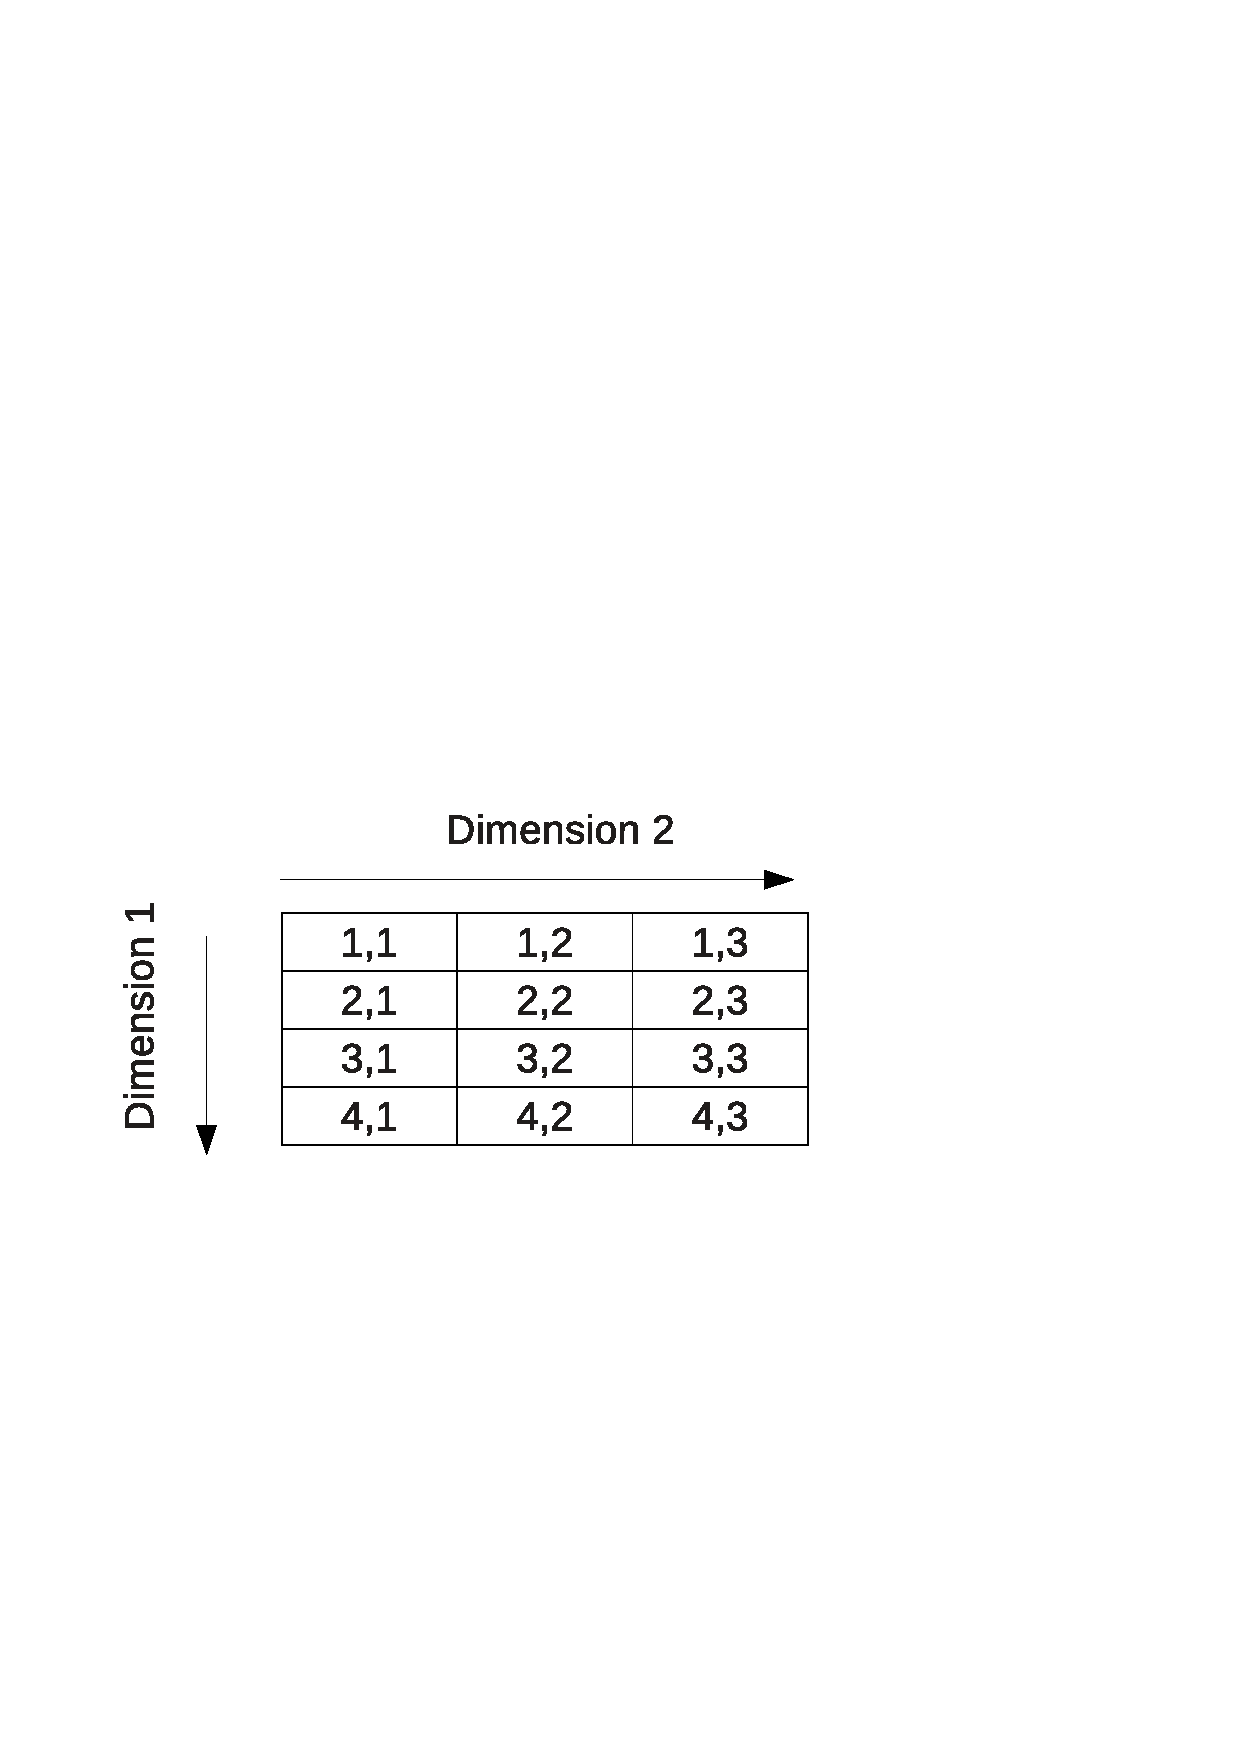
\includegraphics[width=4cm]{./array1}
      \end{center}
      \item Each array has a type and each element of holds a value of that type.
    \end{itemize}
  \end{block}

  \framebreak
  \begin{columns}
    \column{11.5cm}
    \begin{block}{\scriptsize Array Declarations}
      \begin{itemize}
        \item The \texttt{\textbf{dimension}} attribute declares arrays.
        \item Usage: \texttt{\textbf{dimension(lower\_bound:upper\_bound)}}
        \item[] Lower bounds of one \textbf{\texttt{(1:)}} can be omitted
        \item Examples:
        \begin{enumerate}
          \item[$\vardiamond$] \texttt{\textbf{integer, dimension(1:106) ::}} \texttt{atomic\_number}
          \item[$\vardiamond$] \texttt{\textbf{real, dimension(3,0:5,-10:10) ::}} \texttt{values}
          \item[$\vardiamond$] \texttt{\textbf{character(len=3),dimension(12) ::}} \texttt{months} 
        \end{enumerate}
        \item Alternative form for array declaration
        \begin{enumerate}
          \item[$\vardiamond$] \texttt{\textbf{integer ::}} \texttt{days\_per\_week(7), months\_per\_year(12)}
          \item[$\vardiamond$] \texttt{\textbf{real ::}} \texttt{grid(0:100,-100:0,-50:50)}
          \item[$\vardiamond$] \texttt{\textbf{complex ::}} \texttt{psi(100,100)}
        \end{enumerate}
        \item Another alternative form which can be very confusing for readers
        \begin{enumerate}
          \item[$\vardiamond$] \texttt{\textbf{integer, dimension(7) ::}} \texttt{days\_per\_week, months\_per\_year(12)}
        \end{enumerate}
      \end{itemize}
    \end{block}
  \end{columns}
  
  \begin{block}{\scriptsize Array Visualization}
    \begin{itemize}
      \item Define arrays \texttt{a,b,c} and \texttt{d} as follows
      \item[] \textbf{\texttt{real,dimension(15) ::}} \texttt{a}
      \item[] \textbf{\texttt{real,dimension(-4:0,0:2) ::}} \texttt{b}
      \item[] \textbf{\texttt{real,dimension(5,3) ::}} \texttt{c}
      \item[] \textbf{\texttt{real,dimension(4:8,2:4) ::}} \texttt{d}
    \end{itemize}
  \end{block}
  \begin{center}
    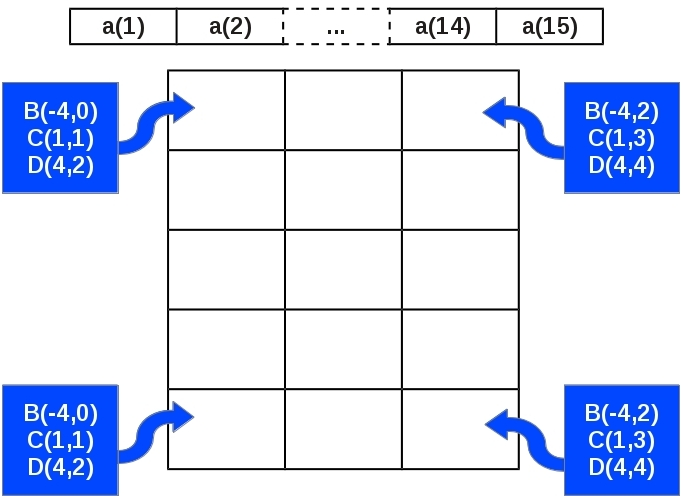
\includegraphics[width=5cm]{./array2-3}
%    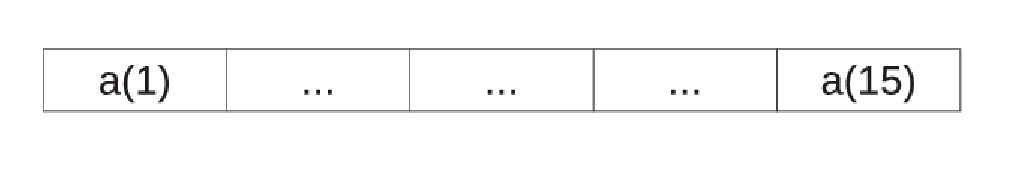
\includegraphics[width=4cm]{./array2}\\
%    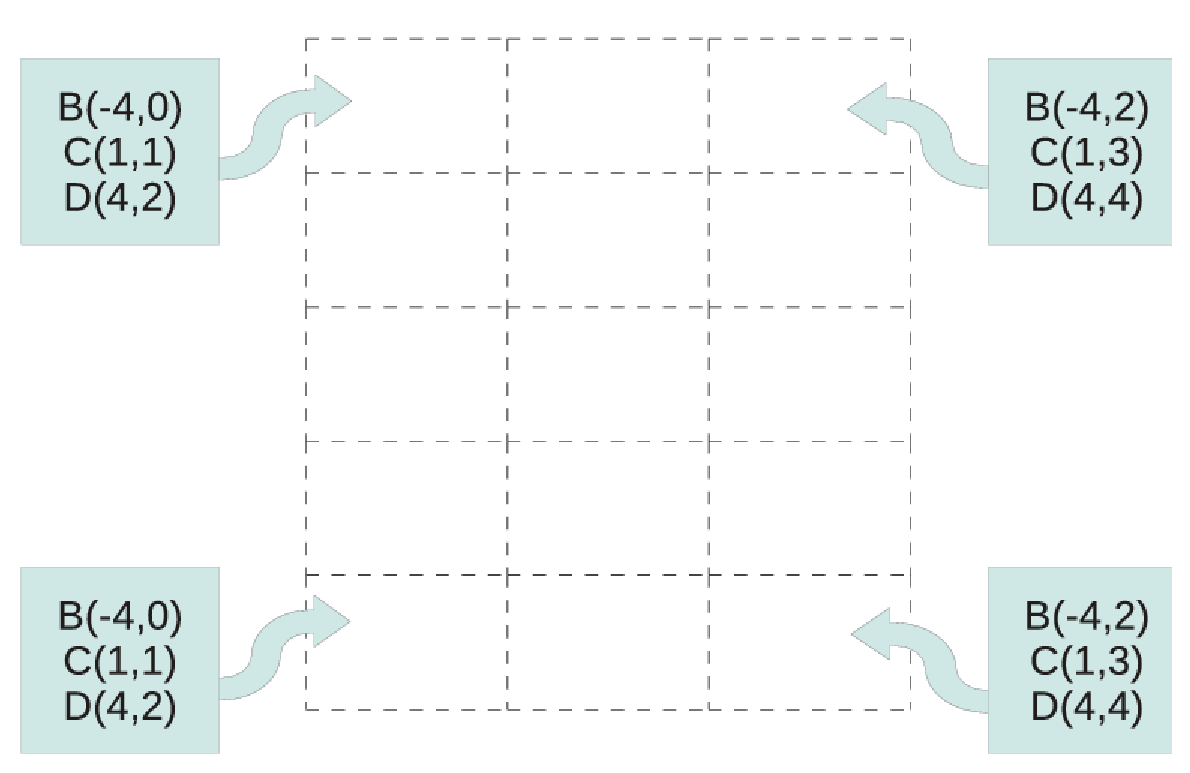
\includegraphics[width=4cm]{./array3}
  \end{center}
  
  \begin{block}{\scriptsize Array Conformance}
    \begin{itemize}
      \item Array or sub-arrays must conform with all other objects in an expression
      \begin{enumerate}
        \item a scalar conforms to an array of any shape with the same value for every element
        \item[] \texttt{c = 1.0} is the same as \texttt{c(:,:) = 1.0}
        \item two array references must conform in their shape.
      \end{enumerate}
    \end{itemize}
  \end{block}
  \begin{center}
    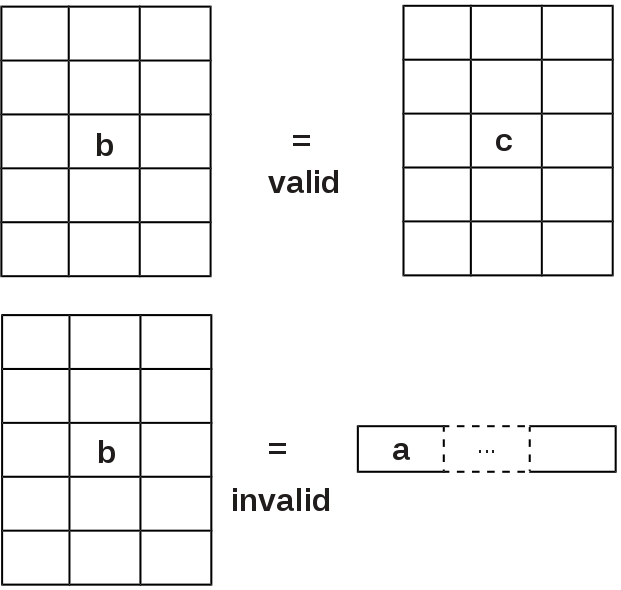
\includegraphics[width=4cm]{./array4}
  \end{center}

  \begin{block}{\scriptsize Array Element Ordering}
    \begin{itemize}
      \item Fortran is a column major form i.e. elements are added to the columns seqeuntially. This ordering can be changed using the \textbf{\texttt{reshape}} intrinsic.
    \end{itemize}
  \end{block}
  \begin{center}
    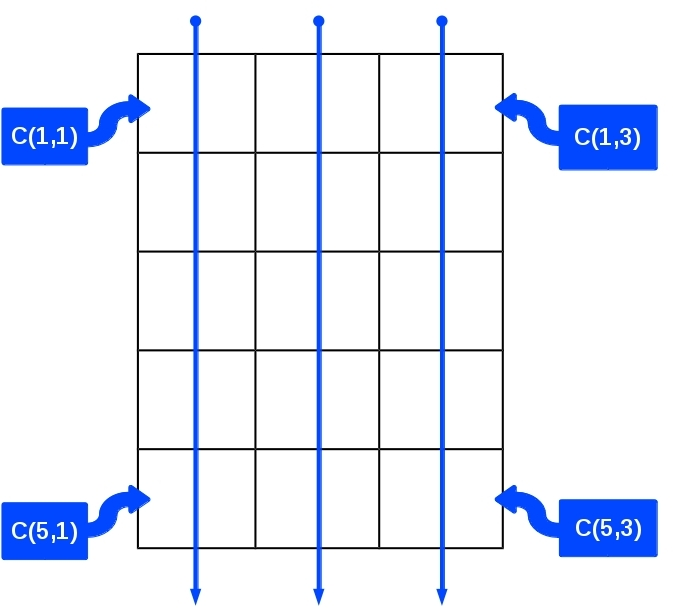
\includegraphics[width=6cm,clip=true]{./array5}
  \end{center}
\end{frame}


\begin{frame}
  \frametitle{\small Array Terminology}
%  \begin{columns}
%    \column{12cm}
    \begin{block}{}
      \begin{itemize}
        \item[] \texttt{\textbf{real ::}} \texttt{a(0:20), b(3,0:5,-10:10)}
      \end{itemize}
      \begin{description}
        \item[Rank:] Number of dimensions.
        \item[] {\texttt{a}} has rank 1 and {\texttt{b}} has rank 3
        \item[Bounds:] upper and lower limits of each dimension of the array.
        \item[] {\texttt{a}} has bounds 0:20 and {\texttt{b}} has bounds 1:3, 0:5 and -10:10
        \item[Extent:] Number of element in each dimension
        \item[] {\texttt{a}} has extent 21 and {\texttt{b}} has extents 3,6 and 21
        \item[Size:] Total number of elements.
        \item[] {\texttt{a}} has size 21 and {\texttt{b}} has 30
        \item[Shape:] The shape of an array is its rank and extent
        \item[] \texttt{a} has shape 21 and \texttt{b} has shape (3,6,21)
      \end{description}
      \begin{itemize}
        \item Arrays are conformable if they share a shape.
        \item The bounds do not have to be the same
        \item[] \texttt{c(4:6) = d(1:3)}
      \end{itemize}
    \end{block}
%  \end{columns}
\end{frame}

\begin{frame}
  \frametitle{\small Array Constructors}
  \begin{itemize}
    \item Used to give arrays or sections of arrays specific values
  \end{itemize}
  \begin{bblock}{}
    {\tiny
      \begin{itemize}
        \item[] \textbf{\texttt{implicit none}}
        \item[] \textbf{\texttt{integer ::}} \texttt{i}
        \item[] \textbf{\texttt{integer, dimension(10) ::}} \texttt{imatrix}
        \item[] \textbf{\texttt{character(len=5),dimension(3) ::}} \texttt{colors}
        \item[] \textbf{\texttt{real, dimension(4) ::}} \texttt{height}
        \item[] \texttt{height = (/5.10, 5.4, 6.3, 4.5 /)}
        \item[] \texttt{colors = (/'red  ', 'green', 'blue ' /)}
        \item[] \texttt{ints = (/ 30, (i = 1, 8), 40 /)}
      \end{itemize}
      }
  \end{bblock}
  \begin{itemize}
    \item constructors and array sections must conform.
    \item[] \texttt{ints = (/ 30, (i = 1, 10), 40/)} is invalid
    \item strings should be padded so that character variables have correct length.
    \item use \textbf{\texttt{reshape}} intrinsic for arrays for higher ranks
    \item \texttt{(i = 1, 8)} is an implied \textbf{\texttt{do}}.
    \item You can also specify a stride in the implied \textbf{\texttt{do}}.
    \item[] \texttt{ints = (/ 30, (i = 1, 16, 2), 40 /)}
    \item {\color{red}There should be no space between / and ( or )}
  \end{itemize}
\end{frame}

\begin{frame}[fragile]
  \frametitle{\small }
  \begin{block}{\scriptsize Reshape}
    \begin{itemize}
      \item \textbf{\texttt{reshape(source, shape, pad, order)}} constructs an array with a specified shape \textbf{\texttt{shape}} starting from the elements in a given array \textbf{\texttt{source}}.  
      \item If \textbf{\texttt{pad}} is not included then the size of \bftt{source} has to be at least \bftt{product (shape)}. 
      \item If \bftt{pad} is included it has to have the same type as \bftt{source}. 
      \item If \bftt{order} is included, it has to be an \bftt{integer} array with the same shape as \bftt{shape} and the values must be a permutation of (1,2,3,...,N), where N is the number of elements in \bftt{shape} , it has to be less than, or equal to 7.
    \end{itemize}
  \end{block}
  \begin{columns}
    \column{2cm}
    {\tiny
      \begin{eblock}{}
        \[ \left( \begin{array}{ccc}
          0 & 0 & 0 \\
          0 & a & a \\
          a & 0 & a \\
          a & a & 0
        \end{array}\right) \]
      \end{eblock}
    }
    \column{4cm}
    {\tiny
      \begin{eblock}{}
        \begin{verbatim}
  rcell = reshape( (/ &
       0.d0, 0.d0, a,    a,   &
       0.d0, a,    0.d0, a,   &
       0.d0, a,    a,    0.d0 &
       /),(/4,3/) )
        \end{verbatim}
      \end{eblock}
    }
    \column{4cm}
    {\tiny
      \begin{eblock}{}
        \begin{verbatim}
  rcell = reshape( (/ &
       0.d0, 0.d0, 0.d0 &
       0.d0, a   , a    &
       a,    0.d0, a    &
       a,    a,    0.d0 &
       /),(/4,3/),order=(/2,1/))
        \end{verbatim}
      \end{eblock}
    }
  \end{columns}
  \vspace{-0.25cm}
  \begin{ablock}{}
    In Fortran, for a multidimensional array, the first dimension has the fastest index while the last dimension has the slowest index i.e. memory locations are continuous for the last dimension. 
    The \bftt{order} statement allows the programmer to change this order. The last example above sets the memory location order which is consistent to that in C/C++.
  \end{ablock}
\end{frame}

\begin{frame}
  \frametitle{\small Array Contructors in Intialization Statements}
  \begin{itemize}
    \item Arrays can be initialized as follows during variable declaration
  \end{itemize}
  \begin{bblock}{}
    {\tiny
      \begin{itemize}
        \item[] \textbf{\texttt{integer, dimension(4) ::}} \texttt{imatrix = (/ 2, 4, 6, 8/)}
        \item[] \textbf{\texttt{character(len=*),dimension(3) ::}} \texttt{colors = (/'red  ', 'green', 'blue '/)}
        \item[] {\color{red}All strings must be the same length}
        \item[] \textbf{\texttt{real, dimension(4) ::}} \texttt{height = (/5.10, 5.4, 6.3, 4.5/)}
        \item[] \textbf{\texttt{integer, dimension(10) ::}} \texttt{ints = (/ 30, (i = 1, 8), 40/)}
        \item[] \textbf{\texttt{real, dimension(4,3), parameter ::}}   \texttt{rcell =} \bftt{reshape}\texttt{( (/0.d0, 0.d0, 0.d0, 0.d0,\&}
        \item[] \texttt{\quad\quad a, a, a,0.d0, a, a, a, 0.d0 /),(/4,3/),}\bftt{order}\texttt{=(/2,1/)) }
      \end{itemize}
    }
  \end{bblock}
\end{frame}

\begin{frame}[allowframebreaks]
  \frametitle{\small Array Syntax}
  \begin{itemize}
    \item whole arrays
    \begin{enumerate}
      \item[$\vardiamond$] \texttt{a = 0.0}
      \item[] sets whole array \texttt{a} to zero
      \item[$\vardiamond$] \texttt{b = c + d}
      \item[] adds \texttt{c} to \texttt{d} and assigns result to \texttt{b}
    \end{enumerate}
    \item elements
    \begin{enumerate}
      \item[$\vardiamond$] \texttt{a(1) = 0.0}
      \item[] sets one element of \texttt{a} to zero
      \item[$\vardiamond$] \texttt{b(1,3) = a(3) + c(5,1)}
      \item[] sets an element of \texttt{b} to the sum of two other array elements.
    \end{enumerate}
    \item array sections
    \begin{enumerate}
      \item[$\vardiamond$] {\texttt{a(0:3) = 5.0}}
      \item[] sets {\texttt{a(0)}}, {\texttt{a(1)}}, {\texttt{a(2)}} and {\texttt{a(3)}} to five
      \item[$\vardiamond$] {\texttt{b(-2:2,4:6) = c(1:5,6:8) + 2.0}}
      \item[] adds two to the subsection of {\texttt{c}} and assigns the result to the subsection of {\texttt{b}}
    \end{enumerate}
    \framebreak
    \item Arrays can be treated as a single variable:
    \begin{enumerate}
      \item[$\vardiamond$] can use intrinsic operators between conformable arrays (or sections)
      \item[] {\texttt{ b = c * d + b**2 }}
      \item[] this is equivalent to
      \item[] {\texttt{ b(-4,0) = c(1,1) * d(4,2) + b(-4,0)**2 }}
      \item[] {\texttt{ b(-3,0) = c(2,1) * d(5,2) + b(-3,0)**2 }}
      \item[] {\texttt{$\cdots$}}
      \item[] {\texttt{ b(-4,0) = c(1,1) * d(4,2) + b(-4,0)**2 }}
      \item[] {\texttt{ b(-4,1) = c(1,2) * d(4,3) + b(-4,1)**2 }}
      \item[] {\texttt{$\cdots$}}
      \item[] {\texttt{ b(-3,2) = c(4,3) * d(7,4) + b(-3,2)**2 }}
      \item[] {\texttt{ b(-4,2) = c(5,3) * d(8,4) + b(-4,2)**2 }}
      \item[]
      \item[$\vardiamond$] elemental intrinsic functions can be used
      \item[] {\texttt{ b = sin(c) + cos(d)}}
      \item[]
      \item[] All operations/functions are applied element by element
    \end{enumerate}
  \end{itemize}
\end{frame}

\begin{frame}[allowframebreaks]
  \frametitle{\small Array Sections}
  \begin{itemize}
    \item[] \textbf{\texttt{real, dimension(6:6) ::}} \texttt{a}
  \end{itemize}
  \begin{columns}
    \column{7cm}
    \begin{itemize}
      \item {\texttt{a(1:3,1:3) = a(1:6:2,2:6:2)}} and
      \item[] {\texttt{a(1:3,1:3) = 1.0 }} are valid
      \item {\texttt{a(2:5,5) = a(2:5,1:6:2)}} and
      \item[] {\texttt{a(2:5,1:6:2) = a(1:6:2,2:6:2)}} are not
      \item {\texttt{a(2:5,5)}} is a 1D section while 
      \item[] {\texttt{a(2:5,1:6:2)}} is a 2D section
    \end{itemize}
    \column{4cm}
    \vspace{-0.5cm}
    \begin{center}
      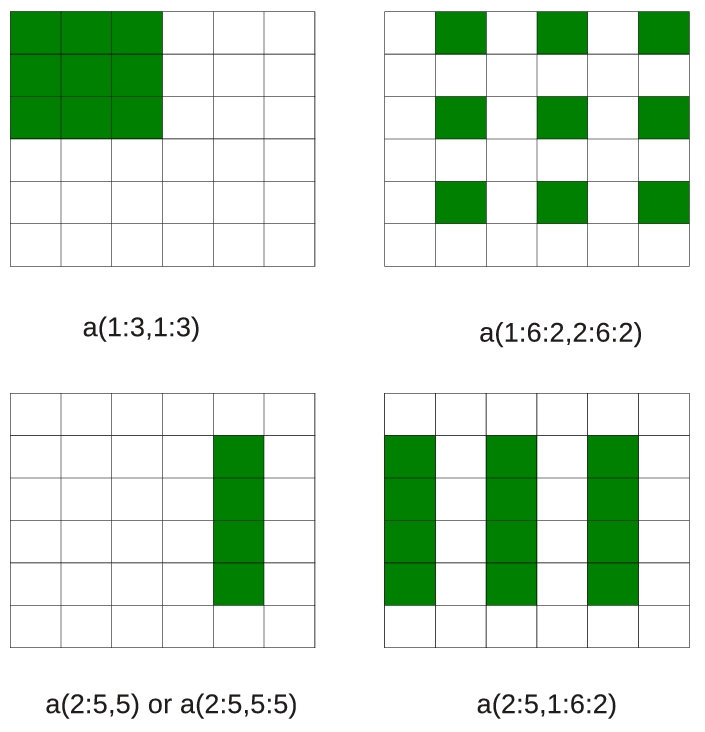
\includegraphics[width=4cm,clip=true]{./array6}
    \end{center}
  \end{columns}

  \begin{itemize}
    \item The general form for specifying sub-arrays or sections is
    \item[] \textit{[<bound1>]:[<bound2>][:<stride>]}
    \item The section starts at \textit{<bound1>} and ends at or before \textit{<bound2>}.
    \item \textit{<stride>} is the increment by which the locations are selected, by default \textit{stride=1}
    \item \textit{<bound1>}, \textit{<bound2>}, \textit{<stride>} must all be scalar integer expressions.
  \end{itemize}

  \begin{bblock}{}
    \begin{itemize}
      \item[] \textbf{\texttt{real, dimension(1:20) ::}} \texttt{a}
      \item[] \textbf{\texttt{integer ::}} \texttt{m,n,k}
    \end{itemize}
    \begin{center}
      \begin{tabular}{lcl}
        {\texttt{a(:)}} &  & the whole array \\
        {\texttt{a(3:9)}} &  & elements 3 to 9 in increments of 1 \\
        {\texttt{a(3:9:1)}} &  & as above \\
        {\texttt{a(m:n)}} &  & elements m through n\\
        {\texttt{a(m:n:k)}} &  & elements m through n in increments of k \\
        {\texttt{a(15:3:-2)}} &  & elements 15 through 3 in increments of -2 \\
        {\texttt{a(15:3)}} &  & zero size array \\
        {\texttt{a(m:)}} &  & elements m through 20, default upper bound \\
        {\texttt{a(:n)}} &  & elements 1, default lower bound through n \\
        {\texttt{a(::2)}} &  & all elements from lower to upper bound in increments of 2 \\
        {\texttt{a(m:m)}} &  & 1 element section \\
        {\texttt{a(m)}} &  & array element not a section \\
        are valid sections. & & \\
      \end{tabular}
    \end{center}
  \end{bblock}
\end{frame}

\begin{frame}[allowframebreaks]
  \frametitle{\small Array I/O}
  \begin{itemize}
    \item[] \textbf{\texttt{real,dimension(4,4) ::}} \texttt{a}
    \item Arrays are printed in the order that they appear in memory
    \item[$\vardiamond$] {\texttt{print *, a}}
    \item[] would produce on output
    \item[] {\texttt{a(1,1),a(2,1),a(3,1),a(4,1),a(1,2),a(2,2),$\cdots$,a(3,4),a(4,4)}}
    \item[$\vardiamond$] {\texttt{read *, a}}
    \item[] would read from input and assign array elements in the same order as above
    \item The order of array I/O can be changed using intrinsic functions such as \bftt{reshape, transpose} or \bftt{cshift}.
  \end{itemize}
  \begin{bblock}{Example}
    \begin{itemize}
      \item Consider a 3x3 matrix
      \begin{center}
        \begin{tabular}{|c|c|c|}
          \hline
          1 & 4 & 7 \\ \hline
          2 & 5 & 8 \\ \hline
          3 & 6 & 9 \\ \hline
        \end{tabular}
      \end{center}
      \item The following print statements
      \item[] {\texttt{ print *, 'array element   = ',a(3,3)}}
      \item[] {\texttt{ print *, 'array section   = ',a(:,2)}}
      \item[] {\texttt{ print *, 'sub-array       = ',a(:3,:2)}}
      \item[] {\texttt{ print *, 'whole array     = ',a}}
      \item[] {\texttt{ print *, 'array transpose = ',transpose(a)}}
      \item would produce the following output
      \item[] array element   = 9
      \item[] array section   = 4 5 6
      \item[] sub-array       = 1 2 3 4 5 6
      \item[] whole array     = 1 2 3 4 5 6 7 8 9
      \item[] array transpose = 1 4 7 2 5 8 3 6 9
    \end{itemize}
  \end{bblock}  
\end{frame}

\begin{frame}[allowframebreaks]
  \frametitle{\small Array Intrinsic Functions}
  \begin{block}{}
    \begin{description}
      \item[{size(x[,n])}] The size of x (along the $n^{th}$ dimension, optional)
      \item[shape(x)] The shape of x
      \item[{lbound(x[,n])}] The lower bound of x
      \item[{ubound(x[,n])}] The upper bound of x
      \item[minval(x)] The minimum of all values of x
      \item[maxval(x)] The maximum of all values of x
      \item[minloc(x)] The indices of the minimum value of x
      \item[maxloc(x)] The indices of the maximum value of x
    \end{description}
  \end{block}
  \begin{block}{}
    \begin{description}
      \item[{sum(x[,n])}] The sum of all elements of x (along the $n^{th}$ dimension, optional)
      \item[] $sum(x) = \sum_{i,j,k,\cdots}x_{i,j,k,\cdots}$
      \item[{product(x[,n])}] The product of all elements of x (along the $n^{th}$ dimension, optional)
      \item[] $prod(x) = \prod_{i,j,k,\cdots}x_{i,j,k,\cdots}$
      \item[transpose(x)] Transpose of array x: $ x_{i,j}\Rightarrow x_{j,i}$
      \item[dot\_product(x,y)] Dot Product of arrays x and y: $ \sum_{i} x_i* y_i $
      \item[matmul(x,y)] Matrix Multiplication of arrays x and y which can be 1 or 2 dimensional arrays: $ z_{i,j} = \sum_k x_{i,k} * y_{k,j}$
      \item[conjg(x)] Returns the conjugate of x: $ a + \imath b \Rightarrow a - \imath b$
    \end{description}
  \end{block}
\end{frame}

\begin{frame}[allowframebreaks]
  \frametitle{\small Allocatable Arrays}
  \begin{block}{\scriptsize Why?}
    \begin{itemize}
      \item At compile time we may not know the size an array needs to be
      \item We may want to change the problem size without recompiling
      \item The molecular dynamics code was written for 108 atoms. If you want to run a simulation for 256 and 1024 atoms, do you need to recompile and create two executables?
    \end{itemize}
  \end{block}
  \begin{block}{}
    \begin{itemize}
      \item Allocatable arrays allow us to set the size at run time.
      \item[] \textbf{\texttt{real, allocatable ::}} \texttt{force(:,:)}
      \item[] \textbf{\texttt{real, dimension(:),allocatable ::}} \texttt{vel}
      \item We set the size of the array using the allocate statement.
      \item[] \textbf{\texttt{allocate}}\texttt{(force(natoms,3))}
      \item We may want to change the lower bound for an array
      \item[] \textbf{\texttt{allocate}}\texttt{(grid(-100,100))}
      \item We may want to use an array once somewhere in the program, say during initialization. Using allocatable arrays also us to dynamically create the array when needed and when not in use, free up memory using the \textbf{\texttt{deallocate}} statement
      \item[] \textbf{\texttt{deallocate}}\texttt{(force,grid)}
    \end{itemize}
  \end{block}
  \begin{block}{}
    \begin{itemize}
      \item Sometimes, we want to check whether an array is allocated or not at a particular part of the code
      \item Fortran provides an intrinsic function, \textbf{\texttt{allocated}} which returns a scalar logical value reporting the status of an array
      \item[] \textbf{\texttt{if ( allocated}}\texttt{(grid)}\bftt{)deallocate}\texttt{(grid)}
      \item[] \textbf{\texttt{if ( .not. allocated}}\texttt{(force)}\bftt{) allocate}\texttt{(force(natoms,3))}
    \end{itemize}
  \end{block}
\end{frame}

\begin{frame}[fragile]
  \frametitle{\small Masked Array Assignment: Where Statement}
  \begin{block}{}
    \begin{itemize}
      \item Masked array assignment is achieved using the \textbf{\texttt{where}} statement
      \item[] \textbf{\texttt{where}} \texttt{( c < 2 ) a = b/c }
      \item[] the left hand side of the assignment must be array valued.
      \item[] the mask, (logical expression) and the right hand side of the assignment must all conform
      \item Fortran 95/2003 introduced the \textbf{\texttt{where ... elsewhere ... end where}} functionality
      \item \textbf{\texttt{where}} statement cannot be nested
    \end{itemize}
  \end{block}
  {\tiny
    \begin{columns}
      \column{5cm}
      \begin{eblock}{MD code: subroutine integrate}
        \begin{verbatim}
     where ( r > boxl ) 
     r = r - boxl
     end where
     where ( r < 0d0 )
        r = r + boxl
     end where
        \end{verbatim}
      \end{eblock}
      \column{5cm}
      \begin{eblock}{original code: subroutine integrate}
        \begin{verbatim}
     do j=1,3
        if (r(j) .gt. boxl(j)) then
           r(j) = r(j) - boxl(j)
        endif
        
        if (r(j) .lt. 0.d0) then
           r(j) = r(j) + boxl(j)
        endif
     enddo
  enddo
        \end{verbatim}
      \end{eblock}
    \end{columns}
  }
\end{frame}

\begin{frame}
  \frametitle{\small Vector valued subscripts}
  \begin{itemize}
    \item A 1D array can be used to subscript an array in a dimension
    \item[] \textbf{\texttt{real, dimension(15) ::}} \texttt{a}
    \item[] \textbf{\texttt{integer, dimension(5) ::}} \texttt{v = (/ 1,4,8,10,15/)}
    \item[] \textbf{\texttt{integer, dimension(3) ::}} \texttt{w = (/ 1,2,3/)}
    \item[$\vardiamond$] {\texttt{a(v)}} is {\texttt{a(1), a(4), a(8), a(10)}} and {\texttt{a(15)}}
    \item[$\vardiamond$] {\texttt{a(v) = 1.2}} is valid
    \item[$\vardiamond$] only 1D vector subscripts are allowed
    \item[] {\texttt{a(1) = prod(c(v,w))}}
  \end{itemize}
\end{frame}

\begin{frame}
  \begin{center}
%    {\fontsize{300}{300}
      \Huge{\textbf{Break}}
%    }
  \end{center}
\end{frame}
\section{Procedures}
\begin{frame}[fragile,allowframebreaks]
  \frametitle{\small Program Units}

  \begin{itemize}
    \item Most programs are hundreds or more lines of code.
    \item Use similar code in several places.
    \item A single large program is extremely difficult to debug and maintain.
    \item Solution is to break up code blocks into procedures
    \begin{description}
      \item[Subroutines:] Some out-of-line code that is called exactly where it is coded
      \item[Functions:] Purpose is to return a result and is called only when the result is needed
      \item[Modules:] A module is a program unit that is not executed directly, but contains data specifications
and procedures that may be utilized by other program units via the use statement.
    \end{description}
  \end{itemize}

  \framebreak

  \begin{columns}
    \column{4.2cm}
    {\tiny
      \begin{bblock}{}
        \begin{verbatim}
program main

  use module1

  implicit none
  variable declarations


  ...
  call routine1(arg1,arg2,arg3)
  ...
  abc = func(arg1,arg2)
  ...

  contains

    subroutine routine1(arg1,arg2)
      ...
    end subroutine routine1

    function func(arg1,arg2)
      ...
    end function func

  end program main
        \end{verbatim}
      \end{bblock}
    }
    \column{6cm}
    {\tiny
      \begin{bblock}{}
        \begin{verbatim}
program name

  specify which modules to use

  variable declarations


  block of statements
  
  call subroutine routine1 with arguments
  block of statements
  abc is some function of arg1 and arg2
  block of statements

  contains internal procedures described below

    contents of subroutine routine1
      ...
    

    contents of function func
      ...


  last end statement
        \end{verbatim}
      \end{bblock}
    }
  \end{columns}

  \framebreak

  {\fontsize{4}{5}
    \begin{columns}
      \column{5.5cm}
      \begin{eblock}{MD Main Program}
        \begin{verbatim}
program md
  use param

  implicit none
  integer :: k, iseed(1)
  real(dp) :: pener,v2t,etot,avtemp
  real(dp),dimension(:,:),allocatable :: coord,coord0,vel,force

  interface
     subroutine setup(coord,vel,coord0)   
       use param,only:dp
       implicit none
       real(dp),dimension(:,:),intent(out) :: coord,coord0,vel
     end subroutine setup
     subroutine verlet(coord,force,pener)
       use param,only:dp
       implicit none
       real(dp),dimension(:,:),intent(in) :: coord
       real(dp),dimension(:,:),intent(out) :: force
       real(dp),intent(out) :: pener
     end subroutine verlet
     subroutine integrate(coord,force,coord0,vel)
       use param,only:dp
       implicit none
       real(dp),dimension(:,:),intent(inout)::coord,coord0,vel
       real(dp),dimension(:,:),intent(in)::force
     end subroutine integrate
     subroutine rescale(vel)
       use param,only:dp
       implicit none
       real(dp),dimension(:,:),intent(inout) :: vel
     end subroutine rescale
  end interface
        \end{verbatim}
      \end{eblock}
      \column{5.5cm}
      \begin{eblock}{}
        \begin{verbatim}
  inp=40
  outp=50
  
  iseed(1) = 12345
  call random_seed
  call random_seed(size=k)
  call random_seed(put=iseed(1:k))
  call init
  iprint = nstep / 10
  allocate(coord(npart,3),coord0(npart,3),vel(npart,3),force(npart,3))
  call setup(coord,vel,coord0)   
  do istep = 1,nstep
     call verlet(coord,force,pener)
     call integrate(coord,force,coord0,vel)
     v2t = 0.d0
     !   Can you use intrinsic functions to simplify this calculation
     do i=1,npart
        v2t = v2t + dot_product(vel(i,:),vel(i,:))
     enddo
     etot = pener + 0.5d0*v2t
     avtemp = v2t / real(3 * npart, dp )
     ! output energies/velocities, deal with this later
     write(44,1000)real(istep,dp)*tstep,pener,v2t,etot,avtemp
     !        if (istep .gt. iprint) then
     !           if (mod(istep,500) .eq. 0) then
     call rescale(vel)
     !           endif   
     !        endif
1000 format(5(1x,1pe15.8,1x))
  enddo
end program md
        \end{verbatim}
      \end{eblock}
    \end{columns}
  }
\end{frame}

\begin{frame}[fragile, allowframebreaks]
  \frametitle{\small Subroutines}

  \begin{block}{\scriptsize CALL Statement}
    The \texttt{\textbf{call}} statement evaluates its arguments and transfers control to the subroutine\\
    Upon return, the next statement is executed.
  \end{block}
  \begin{block}{\scriptsize SUBROUTINE Statement}
    The \texttt{\textbf{subroutine}} statement declares the procedure and its arguments.\\
    These are also known as dummy arguments.
  \end{block}
  \begin{block}{}
    The subroutine's interface is defined by
    \begin{itemize}
      \item The \texttt{\textbf{subroutine}} statement itself
      \item The declarations of its dummy arguments
      \item Anything else that the subroutine uses
      \item In the previous example, the \textbf{\texttt{subroutine verlet}} is an external procedure and can be called by any program unit with the program.
    \end{itemize}
  \end{block}
  \begin{block}{\scriptsize Statement Order}
    \begin{enumerate}
      \item A \texttt{\textbf{subroutine}} statement starts a subroutine
      \item Any \texttt{\textbf{use}} statements come next
      \item \texttt{\textbf{implicit none}} comes next, followed by
      \item rest of the declarations,
      \item executable statements
      \item End with a \texttt{\textbf{end subroutine}} statement
    \end{enumerate}
  \end{block}
  \begin{block}{\scriptsize Dummy Arguments}
    \begin{itemize}
      \item Their names exist only in the procedure and are declared as local variables.
      \item The dummy arguments are associated with the actual arguments passed to the subroutines.
      \item The dummy and actual argument lists must match, i.e. the number of arguments must be the same and each argument must match in type and rank.
    \end{itemize}
  \end{block}
  \framebreak
  {\fontsize{4}{5}
    \begin{columns}
      \column{4.5cm}
      \begin{eeblock}{Example}
        \begin{verbatim}
subroutine verlet(coord_t,force_t,pener)

  use param,only : dp,npart,boxl
  use lennjones

  implicit none
  integer :: i,j
  real(dp) :: f(3),r(3)
  real(dp),dimension(:,:),intent(in) :: coord_t
  real(dp),dimension(:,:),intent(out) :: force_t
  real(dp),intent(out) :: pener
  
  pener = 0.d0
  force_t = 0d0
  
  do i=1,npart-1
     do j=i+1,npart
        r(:) = coord_t(i,:) - coord_t(j,:)
        !
        ! periodic boundary conditions
        !
        r(:) = r(:) - nint(r(:)/boxl(:))*boxl(:)
        !
        ! calculate lennard-jones forces and energies
        !
        r2 = 1.0d0 / (r(1)*r(1) + r(2)*r(2) + r(3)*r(3))
        r6 = r2 * r2 * r2

        f(:) = dvdr(r2,r6)*r(:)
        force_t(i,:) = force_t(i,:) + f
        force_t(j,:) = force_t(j,:) - f
        pener = pener + epot(r2,r6)

     enddo
  enddo
end subroutine verlet
       \end{verbatim}
      \end{eeblock}
      \column{6.5cm}
      \begin{eblock}{How It's Called}
        \begin{verbatim}
program md

  use param
  implicit none
  integer :: k,iseed(1)
  real(dp) :: pener,v2t,etot,avtemp
  real(dp),dimension(:,:),allocatable :: coord,coord0,vel,force

  interface
     ...
     subroutine verlet(coord,force,pener)
       use param,only:dp
       implicit none
       real(dp),dimension(:,:),intent(in) :: coord
       real(dp),dimension(:,:),intent(out) :: force
       real(dp),intent(out) :: pener
     end subroutine verlet
     ...
  end interface
  
  inp=40
  outp=50
  
  iseed(1) = 12345
  call random_seed
  call random_seed(size=k)
  call random_seed(put=iseed(1:k))
  call init
  iprint = nstep / 10
  allocate(coord(npart,3),coord0(npart,3),vel(npart,3),force(npart,3))
  call setup(coord,vel,coord0)   
  do istep = 1,nstep
     call verlet(coord,force,pener)
     call integrate(coord,force,coord0,vel)
     ...
  enddo
end program md

       \end{verbatim}
      \end{eblock}
    \end{columns}
  }
\end{frame}

\begin{frame}
  \frametitle{\small Internal Procedures}
  \begin{itemize}
    \item Internal procedures appear just before the last \textbf{\texttt{end}} statement and are preceeded by the \textbf{\texttt{contains}} statement.
    \item Internal procedures can be either subroutines or functions which can be accessed only by the program, subroutine or module in which it is present
    \item Internal procedures have declaration of variables passed on from the parent program unit
    \item If an internal procedure declares a variable which has the same name as a variable from the parent program unit then this supersedes the variable from the outer scope for the length of the procedure.
%    \item i.e. internal procedures are not global and connot be called by other program units.
  \end{itemize}
\end{frame}

\begin{frame}[fragile]%,allowframebreaks]
  \frametitle{\small Functions}
  \begin{block}{}
    \begin{itemize}
      \item \textbf{\texttt{function}}s operate on the same principle as \textbf{\texttt{subroutine}}s
      \item The only difference is that \textbf{\texttt{function}} returns a value and does not require the \textbf{\texttt{call}} statement 
    \end{itemize}
  \end{block}
  {\fontsize{4}{5}
    \begin{columns}
      \column{5.5cm}
      \begin{eblock}{Example}
        \begin{verbatim}
module lennjones
  use precision
  implicit none
  real(dp) :: d2,d6
  
  contains
    function dvdr(d2,d6) 
      implicit none
      real(dp) :: dvdr
      dvdr = 48*d2*d6*(d6 - 0.5d0)
    end function dvdr
    function epot(d2,d6)
      implicit none
      real(dp) :: epot
      epot = 4.d0*d6*(d6 - 1.d0)
    end function epot
end module lennjones
        \end{verbatim}
      \end{eblock}
      \column{5.5cm}
      \begin{eblock}{How It's Called}
        \begin{verbatim}
subroutine verlet(coord,force,pener)
  use param,only : dp,npart,boxl
  use lennjones

  implicit none
  integer :: i,j
  real(dp) :: f(3),r(3)
  real(dp),dimension(:,:),intent(in) :: coord
  real(dp),dimension(:,:),intent(out) :: force
  real(dp),intent(out) :: pener
  
  pener = 0.d0
  force = 0d0
  do i=1,npart-1
     do j=i+1,npart
        r(:) = coord(i,:) - coord(j,:)
        !     periodic boundary conditions
        r(:) = r(:) - nint(r(:)/boxl(:))*boxl(:)
        !     calculate lennard-jones forces and energies
        r2 = 1.0d0 / (r(1)*r(1) + r(2)*r(2) + r(3)*r(3))
        r6 = r2 * r2 * r2

        f(:) = dvdr(r2,r6)*r(:)
        force(i,:) = force(i,:) + f
        force(j,:) = force(j,:) - f
        pener = pener + epot(r2,r6)
     enddo
  enddo
end subroutine verlet
        \end{verbatim}
      \end{eblock}
    \end{columns}
  }
\end{frame}

\begin{frame}[fragile]%,allowframebreaks]
  \frametitle{\small Array-valued Functions}
  \begin{bblock}{}
    \begin{itemize}
      \item \textbf{\texttt{function}} can also return arrays
    \end{itemize}
  \end{bblock}
  {\fontsize{4}{5}
    \begin{columns}
      \column{5.5cm}
      \begin{eeblock}{Example}
        \begin{verbatim}
module lennjones
  use precision
  implicit none
  real(dp) :: d2,d6
  
  contains
    function dvdr(r,d2,d6)
      implicit none
      real(dp),dimension(:),intent(in) :: r
      real(dp),dimension(size(r,1)) :: dvdr
      real(dp) :: dvr
      dvr = 48*d2*d6*(d6 - 0.5d0)
      dvdr = dvr * r
    end function dvdr
    function epot(d2,d6)
      implicit none
      real(dp) :: epot
      epot = 4.d0*d6*(d6 - 1.d0)
    end function epot
end module lennjones
        \end{verbatim}
      \end{eeblock}
      \column{5.5cm}
      \begin{eeblock}{How It's Called}
        \begin{verbatim}
subroutine verlet(coord,force,pener)
  use param,only : dp,npart,boxl
  use lennjones

  implicit none
  integer :: i,j
  real(dp) :: f(3),r(3)
  real(dp),dimension(:,:),intent(in) :: coord
  real(dp),dimension(:,:),intent(out) :: force
  real(dp),intent(out) :: pener
  
  pener = 0.d0
  force = 0d0
  do i=1,npart-1
     do j=i+1,npart
        r(:) = coord(i,:) - coord(j,:)
        !     periodic boundary conditions
        r(:) = r(:) - nint(r(:)/boxl(:))*boxl(:)
        !     calculate lennard-jones forces and energies
        r2 = 1.0d0 / (r(1)*r(1) + r(2)*r(2) + r(3)*r(3))
        r6 = r2 * r2 * r2

        force(i,:) = force(i,:) + dvdr(r,r2,r6)
        force(j,:) = force(j,:) - dvdr(r,r2,r6)
        pener = pener + epot(r2,r6)
     enddo
  enddo
end subroutine verlet
        \end{verbatim}
      \end{eeblock}
    \end{columns}
  }
\end{frame}

\begin{frame}[fragile]
  \frametitle{\small Recursive Procedures}
  \begin{itemize}
    \item In Fortran 90, recursion is supported as a feature
    \begin{enumerate}
      \item \textbf{\texttt{recursive}} procedures call themselves
      \item \textbf{\texttt{recursive}} procedures must be declared explicitly
      \item \textbf{\texttt{recursive function}} declarations must contain a \textbf{\texttt{result}} keyword, and 
      \item one type of declaration refers to both the function name and the result variable.
    \end{enumerate}
  \end{itemize}    
  {\fontsize{4}{5}
    \begin{columns}
      \column{6cm}
      \begin{eblock}{}
        \begin{verbatim}
program fact

  implicit none
  integer :: i
  print *, 'enter integer whose factorial you want to calculate'
  read *, i

  print '(i5,a,i20)', i, '! = ', factorial(i)

contains
  recursive function factorial(i) result(i_fact)
    integer, intent(in) :: i
    integer :: i_fact

    if ( i > 0 ) then
       i_fact = i * factorial(i - 1)
    else
       i_fact = 1
    end if
  end function factorial

end program fact
        \end{verbatim}
      \end{eblock}
      \column{5cm}
      \begin{beblock}{}
        \begin{verbatim}
[apacheco@qb4 examples] ./factorial
 enter integer whose factorial you want to calculate
10 
   10! =              3628800
[apacheco@qb4 examples] ./fact1
 Enter an integer < 15
10
  10!=        3628800
        \end{verbatim}
      \end{beblock}
    \end{columns}
  }
\end{frame}

\begin{frame}
  \frametitle{\small Argument Association}
  \begin{itemize}
    \item Recall from MD code example the invocation
    \item[] \textbf{\texttt{call subroutine}} \texttt{verlet(coord,force,pener)}
    \item and the subroutine declaration
    \item[] \textbf{\texttt{subroutine}} \texttt{verlet(coord\_t,force\_t,pener)}
    \item[]
    \item {\texttt{coord}} is an actual argument and is associated with the dummy argument {\texttt{coord\_t}}
    \item In {\texttt{subroutine verlet}}, the name {\texttt{coord\_t}} is an alias for {\texttt{coord}}
    \item If the value of a dummy argument changes, then so does the value of the actual argument
    \item Also, recall the {\texttt{dvdr}} function on the previous slide.
    \item {\color{red}The actual and dummy arguments must correspond in type, kind and rank.}
  \end{itemize}
\end{frame}

\begin{frame}[fragile]
  \frametitle{\small Local Objects}
  \begin{columns}
    \column{6cm}
    \begin{itemize}
      \item In \textbf{\texttt{subroutine}} \texttt{verlet},
      \item[] {\texttt{i,j,r}} and {\texttt{f}} are local objects.
      \item Local Objects 
      \begin{enumerate}
        \item[$\vardiamond$] are created each time a procedure is invoked
        \item[$\vardiamond$] are destroyed when the procedure completes
        \item[$\vardiamond$] do not retain their values between calls
        \item[$\vardiamond$] do not exist in the programs memory between calls.
      \end{enumerate}
    \end{itemize}
      \column{4.5cm}
  {\fontsize{4}{5}
      \begin{eblock}{Example}
        \begin{verbatim}
subroutine verlet(coord,force,pener)

  use param,only : dp,npart,boxl
  use lennjones

  implicit none
  integer :: i,j
  real(dp) :: f(3),r(3)
  real(dp),dimension(:,:),intent(in) :: coord
  real(dp),dimension(:,:),intent(out) :: force
  real(dp),intent(out) :: pener
  
  ...

end subroutine verlet
       \end{verbatim}
      \end{eblock}
  }
    \end{columns}
\end{frame}

\begin{frame}[fragile]
  \frametitle{\small Keyword Arguments}

  \begin{block}{}
    \begin{itemize}
      \item Keyword Arguments
      \begin{itemize}
        \item allow arguments to be specified in any order
        \item makes it easy to add an extra argument - no need to modify any calls
        \item helps improve readability of the program
        \item are used when a procedure has optional arguments
      \end{itemize}
      \item once a keyword is used, all subsequent arguments must be keyword arguments
      \item if used with external procedures then the \textbf{\texttt{interface}} must be explicit within the procedure in which it is invoked.
    \end{itemize}
  \end{block}
  {\fontsize{4}{5}
    \begin{columns}
      \column{5.5cm}
      \begin{eblock}{}
        \begin{verbatim}
subroutine verlet(coord_t,force_t,pener_t)

  ...
  real(dp),intent(in),dimension(:,:) :: coord_t
  real(dp),intent(out),dimension(:,:) :: force_t
  real(dp),intent(out) :: pener_t
  ...
end subroutine force
        \end{verbatim}
      \end{eblock}
      \column{5.5cm}
      \begin{eblock}{}
        \begin{verbatim}
program md
         ...
     call verlet(coord,force,pener)
         ...
end program md
        \end{verbatim}
      \end{eblock}
    \end{columns}
  }
  \begin{itemize}
    \item \textbf{\texttt{program}} \texttt{md} can invoke \textbf{\texttt{subroutine}} \texttt{verlet} using
    \begin{enumerate}
      \item using the positional argument invocation (see right block)
      \item using keyword arguments
      \item[] \textbf{\texttt{call}} \texttt{force(force\_t=force, pener\_t=pener, coord\_t=coord)}
      \item[] \textbf{\texttt{call}} \texttt{force(coord, force\_t=force, pener\_t=pener)}
    \end{enumerate}
  \end{itemize}
\end{frame}

\begin{frame}
  \frametitle{\small Optional Arguments}
  \begin{block}{}
    \begin{itemize}
      \item Optional Arguments
      \begin{itemize}
        \item allow defaults to be used for missing arguments
        \item make some procedures easier to use
      \end{itemize}
      \item once an argument has been omitted all subsequent arguments must be keyword arguments
      \item the \textbf{\texttt{present}} intrinsic can be used to check for missing arguments
      \item if used with external procedures then the \textbf{\texttt{interface}} must be explicit within the procedure in which it is invoked.
    \end{itemize}
  \end{block}
\end{frame}

\begin{frame}
  \frametitle{\small Dummy Array Arguments}
  \begin{itemize}
    \item There are two main types of dummy array argument:
    \begin{enumerate}
      \item \textit{explicit-shape}: all bounds specified
      \begin{itemize}
        \item \textbf{\texttt{real, dimension(4,4), intent(in) ::}} \texttt{explicit\_shape}
        \item[] The actual argument that becomes associated with an explicit shape dummy must conform in size and shape
      \end{itemize}
      \item \textit{assumed-shape}: no bounds specified, all inherited from the actual argument
      \begin{itemize}
        \item \textbf{\texttt{real, dimension(:,:), intent(out) ::}} \texttt{assumed\_shape}
        \item An explicit interface must be provided
      \end{itemize}
    \end{enumerate}
    \item dummy arguments cannot be (unallocated) allocatable arrays.
  \end{itemize}
\end{frame}

\begin{frame}[fragile]
  \frametitle{\small Explicit-shape Arrays}
  {\fontsize{4}{5}
    \begin{columns}
    \column{6cm}
    \begin{eblock}{}
      \begin{verbatim}
program md

  implicit none
  integer :: inp,outp,nstep,istep,iprint,i,j,nunit,npart
  real(kind=8) :: boxl(3),tstep,temp,avtemp
  real(kind=8) :: pener,v2t,etot
  real(kind=8),dimension(:,:),allocatable :: coord,coord0,vel,force
  
  ...
  allocate(coord(npart,3),coord0(npart,3),vel(npart,3),force(npart,3))
  call setup(coord,vel,npart,nunit,boxl,coord0,tstep,temp)   
  ...
end program md
      \end{verbatim}
    \end{eblock}
    \column{5.5cm}
    \begin{eblock}{}
      \begin{verbatim}
subroutine setup(coord,vel,npart,nunit,boxl,coord0,tstep,temp)

  implicit none
  real(kind=8) :: coord(npart,3)
  real(kind=8) :: vel(npart,3)
  real(kind=8) :: coord0(npart,3)
  ...
end subroutine setup
      \end{verbatim}
    \end{eblock}
    \end{columns}
  }
\end{frame}

\begin{frame}[fragile]
  \frametitle{\small Assumed-Shape Arrays}
  {\fontsize{4}{5}
    \begin{columns}
    \column{6cm}
    \begin{eblock}{}
      \begin{verbatim}
program md

  use param

  implicit none
  real(dp) :: pener,v2t,etot,avtemp
  real(dp),dimension(:,:),allocatable :: coord,coord0,vel,force

  interface
     subroutine setup(coord,vel,coord0)   
       use param,only:dp
       implicit none
       real(dp),dimension(:,:),intent(out) :: coord,coord0,vel
     end subroutine setup
     ...
  end interface
  
  ...
  allocate(coord(npart,3),coord0(npart,3),vel(npart,3),force(npart,3))
  call setup(coord,vel,coord0)   
  ...
end program md
      \end{verbatim}
    \end{eblock}
    \column{5.5cm}
    \begin{eblock}{}
      \begin{verbatim}
subroutine setup(coord,vel,coord0)

  use param, only : dp,npart,boxl,tstep,temp,nunit

  implicit none
  real(dp),dimension(:,:),intent(out) :: coord,coord0,vel
  ...
end subroutine setup
      \end{verbatim}
    \end{eblock}
    \end{columns}
  }
  \begin{itemize}
    \item The actual arguments cannot be vector subscribed array.
    \item The actual argument cannot be an assumed-size array
    \item In the procedure, bounds begin at 1
    \item If using external procedure, an explicit interface must be described
  \end{itemize}
\end{frame}

\begin{frame}
  \frametitle{\small Automatic Arrays}
  \begin{itemize}
    \item Automatic Arrays: Arrays which depend on dummy arguments
    \begin{enumerate}
      \item their size is determined by dummy arguments
      \item they cannot have the \textbf{\texttt{save}} attribute or be initialized.
    \end{enumerate}
    \item The \textbf{\texttt{size}} intrinsic or dummy arguments can be used to declare automatic arrays.
  \end{itemize}
  \begin{bblock}{}
    \begin{tabbing}
      \bftt{pr}\=\bftt{ogram} \texttt{main} \\
      \> \bftt{im}\=\bftt{plicit none} \\
      \>\> \bftt{integer ::} \texttt{i,j} \\
      \>\> \bftt{real, dimension(5,6) ::} \texttt{a} \\
      \>\> ... \\
      \>\> \bftt{call} \texttt{routine (a,i,j)} \\
      \>\> ... \\
      \> \bftt{contains} \\
      \>\> \bftt{su}\=\bftt{broutine} \texttt{routine(c,m,n)} \\
      \>\>\>\bftt{integer ::} \texttt{m,n} \\
      \>\>\>\bftt{real, dimension(:,:), intent(inout) ::} \texttt{c}    ! assumed shape array \\
      \>\>\>\bftt{real ::} \texttt{b1(m,n)}                             ! automatic array \\
      \>\>\>\bftt{real, dimension(size(c,1),size(c,3)) ::} \texttt{b2}  ! automatic array \\
      \>\>\> ... \\
      \>\> \bftt{end subroutine} \texttt{routine} \\
      \bftt{end program} \texttt{main} 
    \end{tabbing}
  \end{bblock}
\end{frame}

\begin{frame}
  \frametitle{\small Save Attribute and Arrays}
  \begin{itemize}
    \item Declaring a variable (or array) as \textbf{\texttt{save}} gives it a static storage memory.
    \item i.e information about variables is retained in memory between procedure calls.
  \end{itemize}
  \begin{bblock}{}
    \begin{tabbing}
      \bftt{su}\=\bftt{broutine} \texttt{something(iarg1)} \\
      \> \bftt{im}\=\bftt{plicit none} \\
      \>\>\bftt{integer, intent(in) ::} \texttt{iarg1} \\
      \>\>\bftt{real,dimension(:,:),allocatable,save ::} \texttt{a} \\
      \>\>\bftt{real, dimension(:,:),allocatable ::} \texttt{b} \\
      \>\> ... \\
      \>\> \bftt{if (.not.allocated}\texttt{(a)}\bftt{)allocate}\texttt{(a(i,j))} \\
      \>\> \bftt{allocate}\texttt{(b(j,i))} \\
      \>\> ... \\
      \>\> \bftt{deallocate}\texttt{(b)} \\
      \bftt{end subroutine} \texttt{something}
    \end{tabbing}
  \end{bblock}
  \begin{itemize}
    \item Array {\texttt{a}} is saved when {\texttt{something}} exits.
    \item Array {\texttt{b}} is not saved and needs to be allocated every time in {\texttt{something}}  and deallocated, to free up memory, before {\texttt{something}} exits.
  \end{itemize}
\end{frame}

\begin{frame}[fragile]
  \frametitle{\small Intent}
  \begin{itemize}
    \item \textbf{\texttt{intent}} attribute was introduced in Fortran 90 and is recommended as it
    \begin{enumerate}
      \item allows compilers to check for coding errors
      \item facilitates efficient compilation and optimization
    \end{enumerate}
    \item Declare if a parameter is
    \begin{enumerate}
      \item[$\vardiamond$]Input: \bftt{intent(in)} 
      \item[$\vardiamond$]Output: \bftt{intent(out)}
      \item[$\vardiamond$]Both: \bftt{intent(inout)}
    \end{enumerate}
    \begin{columns}
      \column{11cm}
      {\tiny
        \begin{eblock}{}
          \begin{verbatim}
     subroutine integrate(coord,coord0,force,vel)
       use precision
       implicit none
       real(dp),intent(inout),dimension(:,:) :: coord,coord0
       real(dp),intent(in),dimension(:,:) :: force
       real(dp),intent(out),dimension(:,:) :: vel
       ...
     end subroutine integrate
          \end{verbatim}
        \end{eblock}
      }
    \end{columns}
    \item A variable declared as \textbf{\texttt{intent(in)}} in a procedure cannot be changed during the execution of the procedure (see point 1 above)
  \end{itemize}
\end{frame}

\begin{frame}[fragile,allowframebreaks]
  \frametitle{\small Interfaces}
  \begin{itemize}
    \item The \textbf{\texttt{interface}} statement is the first statement in an interface block.
    \item The \textbf{\texttt{interface}} block is a powerful structure that was introduced in FORTRAN 90.
    \item When used, it gives a calling procedure the full knowledge of the types and characteristics of the dummy arguments that are used inside of the procedure that it references.
    \item This can be a very good thing as it provides a way to execute some safety checks when compiling the program. 
    \item Because the main program knows what argument types should be sent to the referenced procedure, it can check to see whether or not this is the case.
    \item If not, the compiler will return an error message when you attempt to compile the program.
  \end{itemize}
  \framebreak
  {\fontsize{4}{5}
    \begin{columns}
      \column{5.5cm}
      \vspace{-0.4cm}
      \begin{eblock}{}
        \begin{verbatim}
subroutine verlet(coord0,coord,vel,force,pener)
  use param,only : dp,npart,tstep,boxl

  implicit none
  integer :: i,j
  real(dp) :: r(3)
  real(dp),dimension(:,:),intent(inout)::coord,coord0
  real(dp),dimension(:,:),intent(out)::vel,force
  real(dp),intent(out)::pener

  interface
     subroutine pot_force(coord,force,pener)
       use precision
       implicit none
       real(dp),dimension(:,:),intent(in) :: coord
       real(dp),dimension(:,:),intent(out) :: force
       real(dp),intent(out) :: pener
     end subroutine pot_force
  end interface
  ! get potential and force
  call pot_force(coord,force,pener)
  !     update positions using the verlet algorithm
  do i=1,npart
     r(:) = 2*coord(i,:) - coord0(i,:) + force(i,:)*tstep*tstep
     vel(i,:) = (r(:) - coord0(i,:)) / (2*tstep)
     !     periodic boundary conditions
     where ( r > boxl ) 
        r = r - boxl
     end where
     where ( r < 0d0 )
        r = r + boxl
     end where
     !  update coordinates
     coord0(i,:) = coord(i,:)
     coord(i,:) = r(:)
  enddo
  !   output coordinates
  ...
end subroutine verlet
        \end{verbatim}
      \end{eblock}
      \column{5.5cm}
      \vspace{-0.4cm}
      \begin{eblock}{}
        \begin{verbatim}
subroutine pot_force(coord,force,pener)
  use param,only : dp,npart,boxl,pot
  use lennjones

  implicit none
  integer :: i,j
  real(dp) :: f(3),r(3),V
  real(dp),dimension(:,:),intent(in) :: coord
  real(dp),dimension(:,:),intent(out) :: force
  real(dp),intent(out) :: pener
  
  pener = 0.d0
  force = 0d0
  
  do i=1,npart-1
     do j=i+1,npart
        r(:) = coord(i,:) - coord(j,:)
        !     periodic boundary conditions
        r(:) = r(:) - nint(r(:)/boxl(:))*boxl(:)
        !     calculate lennard-jones forces and energies
        select case(pot)
        case("lj", "LJ")
           call ljpot(r,f,V)
        case("mp", "MP")
           call morse(r,f,V)
        case default
           call ljpot(r,f,V)
        end select
        pener = pener + V
        force(i,:) = force(i,:) + f(:)
        force(j,:) = force(j,:) - f(:)
     enddo
  enddo

end subroutine pot_force
        \end{verbatim}
      \end{eblock}
    \end{columns}
  }
  \framebreak
  {\fontsize{4}{5}
    \begin{columns}
      \column{5.5cm}
      \vspace{-0.4cm}
      \begin{eeblock}{}
        \begin{verbatim}
subroutine verlet(coord0,coord,vel,force,pener)
  use param,only : dp,npart,tstep,boxl
  
  implicit none
  integer :: i,j
  real(dp) :: r(3)
  real(dp),dimension(:,:),intent(inout)::coord,coord0
  real(dp),dimension(:,:),intent(out)::vel,force
  real(dp),intent(out)::pener
  
  ! get potential and force
  call pot_force(coord,force,pener)
  !     update positions using the verlet algorithm
  do i=1,npart
     r(:) = 2*coord(i,:) - coord0(i,:) + force(i,:)*tstep*tstep
     vel(i,:) = (r(:) - coord0(i,:)) / (2*tstep)
     !     periodic boundary conditions
     where ( r > boxl ) 
        r = r - boxl
     end where
     where ( r < 0d0 )
        r = r + boxl
     end where
     !  update coordinates
     coord0(i,:) = coord(i,:)
     coord(i,:) = r(:)
  enddo
  !   output coordinates
  
contains
  
        \end{verbatim}
      \end{eeblock}
      \column{5.5cm}
      \vspace{-0.4cm}
      \begin{eeblock}{}
        \begin{verbatim}
  subroutine pot_force(coord,force,pener)
    use lennjones
    
    real(dp) :: f(3),r(3),V
    
    pener = 0.d0
    force = 0d0
    
    do i=1,npart-1
       do j=i+1,npart
          r(:) = coord(i,:) - coord(j,:)
          !     periodic boundary conditions
          r(:) = r(:) - nint(r(:)/boxl(:))*boxl(:)
          !     calculate lennard-jones forces and energies
          select case(pot)
          case("lj", "LJ")
             call ljpot(r,f,V)
          case("mp", "MP")
             call morse(r,f,V)
          case default
             call ljpot(r,f,V)
          end select
          pener = pener + V
          force(i,:) = force(i,:) + f(:)
          force(j,:) = force(j,:) - f(:)
       enddo
    enddo
    
  end subroutine pot_force
  
end subroutine verlet
        \end{verbatim}
      \end{eeblock}
    \end{columns}
  }
  \begin{itemize}
    \item Here since \bftt{subroutine} \texttt{pot\_force} is an internal procedure, no \bftt{interface} is required since it is already implicit and all variable declarations are carried over from \bftt{subroutine} \texttt{verlet}
  \end{itemize}
\end{frame}

\begin{frame}[fragile,allowframebreaks]
  \frametitle{\small Modules}
  \begin{itemize}
%    \item A module is a program unit that is not executed directly, but contains data specifications and procedures that may be utilized by other program units via the use statement.
    \item Modules were introduced in Fortran 90 and have a wide range of applications.
    \item Modules allow the user to write object based code.
    \item A \textbf{\texttt{module}} is a program unit whose functionality can be exploited by other programs which attaches to it via the \textbf{\texttt{use}} statement.
    \item A \textbf{\texttt{module}} can contain the following
    \begin{enumerate}
      \item global object declaration: replaces Fortran 77 COMMON and INCLUDE statements
      \item interface declaration: all external procedures using assumed shape arrrays, intent and keyword/optional arguments must have an explicit interface
      \item procedure declaration: include procedures such as subroutines or functions in modules. Since modules already contain explicit interface, an interface statement is not required
    \end{enumerate}
  \end{itemize}
  \framebreak
  {\fontsize{4}{5}
    \begin{columns}
      \column{5.5cm}
      \vspace{-0.5cm}
      \begin{eblock}{}
        \begin{verbatim}
module precision

  implicit none
  integer,parameter :: dp = selected_real_kind(15)

end module precision

module param
  use precision

  implicit none
  integer :: inp,outp,nstep,istep,i,j,nunit,npart
  real(dp) :: boxl(3),tstep,temp
  character(len=2) :: pot

end module param

module lennjones
  use precision

  implicit none
  real(dp) :: r2,r6,d2,d6
  
  contains 
    subroutine ljpot(r,f,p)
      implicit none
      real(dp),dimension(:),intent(in) :: r
      real(dp),dimension(:),intent(out) :: f
      real(dp),intent(out) :: p

      r2 = 1.0d0 / dot_product(r,r) 
      r6 = r2 * r2 * r2
      
      f(:) = dvdr(r2,r6)*r(:)
      p = epot(r2,r6)      
    end subroutine ljpot
        \end{verbatim}
      \end{eblock}
      \column{5.5cm}
      \vspace{-0.5cm}
      \begin{eblock}{}
        \begin{verbatim}
    subroutine morse(r,f,p)
      implicit none
      real(dp),dimension(:),intent(in) :: r
      real(dp),dimension(:),intent(out) :: f
      real(dp),intent(out) :: p

      f(:) = morseforce(dot_product(r,r))*r(:)
      p = morsepot(dot_product(r,r))
    end subroutine morse
    function dvdr(r2,r6) 
      implicit none
      real(dp) :: dvdr
      real(dp),intent(in) :: r2,r6
      dvdr = 48*r2*r6*(r6 - 0.5d0)
    end function dvdr

    function epot(r2,r6)
      implicit none
      real(dp) :: epot
      real(dp),intent(in) :: r2,r6      
      epot = 4.d0*r6*(r6 - 1.d0)
    end function epot

    function morsepot(d2)
      implicit none
      real(dp),intent(in) :: d2
      real(dp) :: morsepot
      real(dp) :: de,re,a
      de = 0.176d0 ; a = 1.40d0 ; re = 1d0
      morsepot = de * (1d0 - exp(-a*(sqrt(d2)-re)))**2
    end function morsepot

    function morseforce(d2)
      implicit none
      real(dp),intent(in) :: d2
      real(dp) :: morseforce
      real(dp) :: de,re,a,r
      de = 0.176d0 ; a = 1.40d0 ; re = 1d0 ; r = sqrt(d2)
      morseforce = 2d0 * de * a * (1d0 - exp(-a*(r-re)))* &
         exp(-a*(r-re))
    end function morseforce
end module lennjones
        \end{verbatim}
      \end{eblock}
    \end{columns}
  }

  \begin{itemize}
    \item within a \textbf{\texttt{module}}, functions and subroutines are called module procedures.
    \item \textbf{\texttt{module}} procedures can contain internal procedures
    \item \textbf{\texttt{module}} objects that retain their values should be given a \textbf{\texttt{save}} attribute
    \item \textbf{\texttt{module}}s can be used by procedures and other modules, see \textbf{\texttt{module precision}}.
    \item \textbf{\texttt{module}}s can be compiled separately. {\color{red}They should be compiled before the program unit that uses them}.
    \item[] Observe that in my examples with all code in single file, the \textbf{\texttt{module}}s appear before the main program and subroutines.
  \end{itemize}

  \begin{block}{\scriptsize Visibility of module procedures}
    \begin{itemize}
      \item By default, all module procedures are public i.e. they can accessed by program units that use the module using the \textbf{\texttt{use}} statement
      \item To restrict the visibility of the module procedure only to the module, use the \textbf{\texttt{private}} statement
      \item In the \textbf{\texttt{module lennjones}}, all functions which calculate forces can be declared as private as follows
      \begin{columns}
        \column{5cm}
        \begin{eblock}{}
          {\fontsize{4}{5}
          \begin{verbatim}
module lennjones
  use precision

  implicit none
  real(dp) :: r2,r6,d2,d6
  public :: ljpot, morse,epot,moresepot
  private :: dvdr, morseforce
  ...
          \end{verbatim}
          }
        \end{eblock}
      \end{columns}
    \item Program Units in the MD code can directly call \textbf{\texttt{ljpot,morse,epot}} and \textbf{\texttt{moresepot}} but cannot access \textbf{\texttt{dvdr}} and \textbf{\texttt{morseforce}}
    \end{itemize}
  \end{block}
  \begin{block}{\scriptsize \textbf{\texttt{use}} statement}
    \begin{itemize}
      \item The \textbf{\texttt{use}} statement names a module whole public definitions are to be made accessible.
      \item[] To use all variables from \textbf{\texttt{module param}} in \textbf{\texttt{program md}}:
      {\fontsize{4}{5}
        \begin{columns}
          \column{5cm}
          \begin{eblock}{}
            \begin{verbatim}
        program md
          use param
          ...
        end program md
            \end{verbatim}
          \end{eblock}
        \end{columns}
      }
      \item \textbf{\texttt{module}} entities can be renamed
      \item[] To rename \textbf{\texttt{pot}} and \textbf{\texttt{tstep}} to more user readable variables:
      {\fontsize{4}{5}
        \begin{columns}
          \column{5cm}
          \begin{eblock}{}
            \begin{verbatim}
        use param, pot => potential, tstep => timestep
            \end{verbatim}
          \end{eblock}
        \end{columns}
      }
      \item It's good programming practice to use only those variables from \textbf{\texttt{module}}s that are neccessary to avoid name conflicts and overwrite variables.
      \item For this, use the \textbf{\texttt{use <module name>, only}} statement
      {\fontsize{4}{5}
        \begin{columns}
          \column{7cm}
          \begin{eblock}{}
            \begin{verbatim}
        subroutine verlet(coord,force,pener)
          use param,only : dp,npart,boxl,tstep
          ...
        end subroutine verlet
            \end{verbatim}
          \end{eblock}
        \end{columns}
      }
    \end{itemize}
  \end{block}
\end{frame}

\begin{frame}[allowframebreaks]
  \frametitle{\small Compiling Modules}
  \begin{itemize}
    \item Consider the MD code containing a main program \texttt{md.f90}, modules \texttt{precision.f90, param.f90} and \texttt{lennjones.f90} and subroutines \texttt{init.f90, setup.f90, verlet.f90, rescale.f90, gaussran.f90} and \texttt{pot\_force.f90}.
    \item In general, the code can be compiled as 
    \begin{block}{}
      {\tiny
        ifort -o md md.f90 precision.f90 param.f90 lennjones.f90 init.f90 setup.f90 verlet.f90 rescale.f90 gaussran.f90 pot\_force.f90
      }
    \end{block}
    \item Most compilers are more restrictive in the order in which the modules appear.
    \item In general, the order in which the sub programs should be compiled is the following
    \begin{enumerate}
      \item Modules that do not use any other modules.
      \item Modules that use one or more of the modules already compiled.
      \item Repeat the above step until all modules are compiled and all dependencies are resolved.
      \item Main program followed by all subroutines and functions (if any).
    \end{enumerate}
    \item In the MD code, the module \texttt{precision} does not depend on any other modules and should be compiled first
    \item The modules \texttt{param} and \texttt{lennjones} only depend on \texttt{precision} and can be compiled in any order
    \item The main program and subroutines can then be compiled
    \begin{block}{}
      {\tiny
        ifort -o md precision.f90 param.f90 lennjones.f90 md.f90 init.f90 setup.f90 verlet.f90 rescale.f90 gaussran.f90 pot\_force.f90
      }
    \end{block}
    \item modules are designed to be compiled independently of the main program and create a \texttt{.mod} files which need to be linked to the main executable.
    \begin{block}{}
      {\tiny
        ifort -c precision.f90 param.f90 lennjones.f90 \\
        creates precision.mod param.mod lennjones.mod
        }
    \end{block}
    \item The main program can now be compiled as
    \begin{block}{}
      {\tiny
        ifort -o md md.f90 init.f90 setup.f90 verlet.f90 rescale.f90 gaussran.f90 pot\_force.f90 -I\{path to directory containing the .mod files\}
      }
    \end{block}
    \item The next tutorial on Makefiles will cover this aspect in more detail.
  \end{itemize}
\end{frame}

\section{Derived Types and Pointers}
\begin{frame}[fragile,allowframebreaks]
  \frametitle{\small Derived Types}
  \begin{itemize}
    \item Defined by user (also called structures)
    \item Can include different intrinsic types and other derived types
    \item Components are accessed using the percent operator (\%)
    \item Only assignment operator (=) is defined for derived types
    \item Can (re)define operators - see function overloading
    \item Derived type definitions should be placed in a \textbf{\texttt{module}}.
    \item Previously defined type can be used as components of other derived types.
    {\tiny
      \begin{columns}
        \column{6.5cm}
        \begin{bblock}{}
          \begin{tabbing}
            \bftt{ty}\=\bftt{pe line\_type} \\
            \> \bftt{real ::} \texttt{x1, y1, x2, y2} \\
            \bftt{end type line\_type} \\
            \bftt{type (line\_type) ::} \texttt{a, b} \\
            \bftt{type vector\_type} \\
            \> \bftt{type(line\_type) ::} \texttt{line} ! position of center of sphere\\
            \> \bftt{integer ::} \texttt{direction} ! 0=no direction, 1=(x1,y1)->(x2,y2) or 2\\
            \bftt{end type vector\_type} \\
            \bftt{type (vector\_type) ::} \texttt{c, d}
          \end{tabbing}
        \end{bblock}
      \end{columns}
    }
    \framebreak
    \item values can be assigned to derived types in two ways
    \begin{enumerate}
      \item component by component
      \item[] individual component may be selected using the \% operator
      \item as an object
      \item[] the whole object may be selected and assigned to using a constructor
    \end{enumerate}
    {\fontsize{6}{7}
      \begin{bblock}{}
        \texttt{a\%x1 = 0.0 ; a\%x2 = 0.5 ; a\%y1 = 0.0 ; a\%y2 = 0.5} \\
        \texttt{c\%direction = 0} ; \texttt{c\%line\%x1 = 0.0} ; \texttt{c\%line\%x2 = 1.0} ; \texttt{c\%line\%y1 = -1.0} ; \texttt{c\%line\%y2 = 0.0}
      \end{bblock}
      \begin{bblock}{}
        \texttt{b = line\_type(0.0, 0.0, 0.5, 0.5)} \\
        \texttt{d\%line = line\_type(0.0, -1.0, 1.0, 0.0)} \\
        \texttt{d = vector\_type( d\%line, 1 ) or} \\
        \texttt{d = vector\_type( line\_type(0.0, -1.0, 1.0, 0.0), 1)}
      \end{bblock}
    }
    \item Assigment between two objects of the same derived type is intrinsically defined
    \item[] In the previous  example: \texttt{a = b} is allowed but \texttt{a = c} is not.
    {\fontsize{4}{5}
      \begin{columns}
        \column{5.5cm}
        \begin{eblock}{\textbf{\texttt{subroutine setup}}}
          \begin{verbatim}
      coord_t0(pnum+cell)\%x = rcell(cell,1) + real(xx-1,dp)/cells
      coord_t0(pnum+cell)\%y = rcell(cell,2) + real(yy-1,dp)/cells
      coord_t0(pnum+cell)\%z = rcell(cell,3) + real(zz-1,dp)/cells
          \end{verbatim}
        \end{eblock}
        \column{4cm}
        \begin{eeblock}{}
          \begin{verbatim}
      x = rcell(cell,1) + real(xx-1,dp)/cells
      y = rcell(cell,1) + real(yy-1,dp)/cells
      z = rcell(cell,1) + real(zz-1,dp)/cells
      coord_t0(pnum+cell) = dynamics( x, y, z )
          \end{verbatim}
        \end{eeblock}
      \end{columns}
    }
  \end{itemize}
  \framebreak
  \begin{block}{\scriptsize I/O on Derived Types}
    \begin{itemize}
      \item Can do normal I/O on derived types
      \item[] \texttt{print *, a} will produce the result
      \item[] 1.0  0.5  1.5
      \item[] \texttt{print *, c} will produce the result
      \item[] 2.0  0.0  0.0  0.0
    \end{itemize}
  \end{block}
  \framebreak
  \begin{block}{\scriptsize Arrays and Derived Types}
    \begin{itemize}
      \item Can define derived type objects which contain non-allocatable arrays and arrays of derived type objects
    \end{itemize}
  \end{block}

  {\fontsize{4}{5}
    \begin{columns}
      \column{5cm}
      \begin{eblock}{MD code}
        \begin{verbatim}
module dynamic_data
  use precision

  implicit none
  type dynamics
     real(dp) :: x,y,z
  end type dynamics

  type(dynamics),dimension(:),allocatable :: coord,vel,force
end module dynamic_data
        \end{verbatim}
      \end{eblock}
      \column{5cm}
      \begin{ablock}{From one of my old codes}
        \begin{verbatim}
  type atomic
     character(2)::symbol
     real(dp)::mass,charge,alpc,delc,alpd,alpq,betaone,delta
     integer::number,ls_nprime(2,4),n_shell(0:2),&
          prim_counter(0:3,20),npp(0:3),nls(1:3)
     real(dp)::g_exp(20,0:3,6,20),g_coeff(20,0:3,6,20),&
          g_norm(20,0:3,6,20),sr_coef(0:2,4),&
          sr_exp(0:2,4),ls_coef(2,4),ls_exp(2,4),centerdim
  end type atomic
        \end{verbatim}
      \end{ablock}
    \end{columns}
  }
  
  \begin{block}{\scriptsize Derived Type Valued Functions}
    \begin{itemize}
      \item Functions can return results of an arbitrary defined type.
    \end{itemize}
  \end{block}

  \begin{block}{\scriptsize Private Derived Types}
    \begin{itemize}
      \item A derived type can be wholly private or some of its components hidden
      \begin{columns}
        \column{5cm}
        {\tiny
          \begin{bblock}{}
            \begin{tabbing}
              \bftt{mo}\=\bftt{dule} \texttt{data}\\
              \> \bftt{ty}\=\bftt{pe :: position} \\
              \>\> \bftt{real, private ::} \texttt{x,y,z} \\
              \> \bftt{end type position} \\
              \> \bftt{ty}\=\bftt{pe, private :: acceleration} \\
              \>\> \bftt{real ::} \texttt{x,y,z} \\
              \> \bftt{end type acceleration} \\
              \> \bftt{contains} \\
              \>\> ... \\
              \bftt{end module} \texttt{data}
            \end{tabbing}
          \end{bblock}
        }
      \end{columns}
      \item Program units that use \texttt{data} have \texttt{position} exported but not it's components \texttt{x,y,z} and the derived type \texttt{acceleration}
    \end{itemize}
  \end{block}
\end{frame}

\begin{frame}[allowframebreaks]
  \frametitle{\small Pointers}
  \begin{itemize}
    \item In Fortran, a \bftt{pointer} variable or simply a \bftt{pointer} is best thought of as a ``free-floating'' name that may be associated with or ``aliased to'' some object.
    \item The object may already have one or more other names or it may be an unnamed object.
    \item The object represent data (a variable, for example) or be a procedure.
    \item A \bftt{pointer} is any variable that has been given the \bftt{pointer} attribute.
    \item A variable with the \bftt{pointer} attribute may be used like any ordinary variable.
  \end{itemize}

  \begin{block}{}
    Each pointer is in one of the following three states:
    \begin{description}
      \item[undefined] condition of each \bftt{pointer} at the beginning of a \bftt{program}, unless it has been initialized
      \item[null] not an alias of any data object
      \item[associated] it is an alias of some target data object
    \end{description}
  \end{block}
  
  \framebreak
  \begin{block}{}%{\bftt{pointer} declaration and assignment}
    \begin{itemize}
      \item \bftt{pointer} objects must be declared with the \bftt{pointer} attribute
      \item[] \bftt{real, pointer :: } \texttt{p}
      \item Any variable aliased or ``pointed to'' by a \bftt{pointer} must be given the \bftt{target} attribute
      \item[] \bftt{real, target :: } \texttt{r}
      \item To make \texttt{p} an alias to \texttt{r}, use the \bftt{pointer assignment statement}
      \item[] \texttt{p => r}
      \item The variable declared as a \bftt{pointer} may be a simple variable as above, an array or a structure
      \item[] \bftt{real, dimension(:), pointer ::} \texttt{v}
      \item \bftt{pointer} \texttt{v} declared above can now be aliased to a 1D array of reals or a row or column of a multi-dimensional array
      \item[] \bftt{real, dimension(100,100), target ::} \texttt{a}
      \item[] \texttt{v => a(5,:)}
      \item \bftt{pointer} variables can be used as any other variables
      \item[] For example, \texttt{print *, v} and \texttt{print *, a(5,:)} are equivalent
      \item[] \texttt{v = 0.0 } is the same as \texttt{a(5,:) = 0.0'}
    \end{itemize}
  \end{block}
  \begin{itemize}
    \item \bftt{pointer} variables can also be an alias to another \bftt{pointer} variable
  \end{itemize}
  \begin{columns}
    \column{5.5cm}
    \begin{bblock}{}
      \begin{itemize}
        \item Consider the following example
        \item[] \bftt{real, target ::} \texttt{r}
        \item[] \bftt{real, pointer ::} \texttt{p1, p2}
        \item[] \texttt{r = 4.7}
        \item[] \texttt{p1 => r}
        \item[] \texttt{p2 => r}
        \item[] \texttt{print *, r, p1, p2}
        \item[] \texttt{r = 7.4}
        \item[] \texttt{print *, r, p1, p2}
        \item The output on the screen will be
        \item[] 4.7  4.7  4.7
        \item[] 7.4  7.4  7.4
        \item Changing the value of \texttt{r} to 7.4 causes the value of both \texttt{p1} and \texttt{p2} to change to 7.4
      \end{itemize}
    \end{bblock}
    \column{5.5cm}
    \begin{bblock}{}
      \begin{itemize}
        \item Consider the following example
        \item[] \bftt{real, target ::} \texttt{r1, r2}
        \item[] \bftt{real, pointer ::} \texttt{p1, p2}
        \item[] \texttt{r1 = 4.7; r2 = 7.4}
        \item[] \texttt{p1 => r1 ; p2 => r2}
        \item[] \texttt{print *, r1, r2, p1, p2}
        \item[] \texttt{p1 = p2}
        \item[] \texttt{print *, r1, r2, p1, p2}
        \item The output on the screen will be
        \item[] 4.7  7.4  4.7  7.4
        \item[] 4.7  4.7  4.7  4.7
        \item The assignment statement \texttt{p2 = p1} has the same effect of \texttt{r2 = r1} since \texttt{p1} is an alias to \texttt{r1} and \texttt{p2} is an alias to \texttt{r2}
      \end{itemize}
    \end{bblock}
  \end{columns}

  \begin{itemize}
    \item The \bftt{allocate} statement can be used to create space for a value and cause a pointer to refer to that space.
    \item[] \bftt{allocate}\texttt{(p1)} creates a space for one real number and makes \texttt{p1} an alias to that space.
    \item No real value is stored in that space so it is neccessary to assign a value to \texttt{p1}
    \item \texttt{p1 = 4.7} assigns a value 4.7 to that allocated space
    \item Before a value is assigned to \texttt{p1}, it must either be associated with an unnamed target using the \bftt{allocate} statement or be aliased with a target using the pointer assignment statement.
    \item \bftt{deallocate} statement dissociates the pointer from any target and nullifies it
    \item[] \bftt{deallocate}\texttt{(p1)}
  \end{itemize}
\end{frame}

\begin{frame}
  \frametitle{\small Pointer Intrinsic Functions}
  \begin{block}{\scriptsize null intrinsic}
    \begin{itemize}
      \item \bftt{pointer} variables are undefined unless they are initialized
      \item \bftt{pointer} variable must not be reference to produce a value when it is undefined.
      \item It is sometime desirable to have a \bftt{pointer} variable in a state of not pointing to anything
      \item The \bftt{null} intrinsic function nullifies a pointer assignment so that it is in a state of not pointing to anything
      \item[] \texttt{p1 =>} \bftt{null()}
      \item If the target of \texttt{p1} and \texttt{p2} are the same, then nullifying \texttt{p1} does not nullify \texttt{p2}
      \item If \texttt{p1} is null and \texttt{p2} is pointing to \texttt{p1}, then \texttt{p2} is also nullified.
    \end{itemize}
  \end{block}
  \begin{block}{\scriptsize associated intrinsic}
    \begin{itemize}
      \item The \bftt{associated} intrinsic function queries whether a pointer varibale is pointing to, or is an alias for another object.
      \item[] \bftt{associated}\texttt{(p1,r1)} and \bftt{associated}\texttt{(p2,r2)} are true, but
      \item[] \bftt{associated}\texttt{(p1,r2)} and \bftt{associated}\texttt{(p2,r1)} are false
    \end{itemize}
  \end{block}
\end{frame}
\section{Object Based Programming}
\begin{frame}
  \frametitle{\small OOP Concepts}
  \begin{block}{\scriptsize Fortran 90 has some Object Oriented facilites such as}
    \begin{enumerate}
      \item data abstraction: user defined types (covered)
      \item data hiding - private and public attributes (covered)
      \item encapsulation - modules and data hiding facilities (covered)
      \item inheritance and extensibility - super-types, operator overloading and generic procedures
      \item polymorphism - user can program his/her own polymorphism by generic overloading
      \item resuability - modules
    \end{enumerate}
  \end{block}
\end{frame}

\begin{frame}[fragile,allowframebreaks]
  \frametitle{\small Overloading Procedures}
  \begin{itemize}
    \item In Fortran, most intrinsic functions are generic in that their type is determined by their argument(s)
    \item For example, the \bftt{abs}\texttt{(x)} intrinsic function comprises of
    \begin{enumerate}
      \item \bftt{cabs} : called when \texttt{x} is \bftt{complex}
      \item \bftt{abs} : called when \texttt{x} is \bftt{real}
      \item \bftt{iabs} : called when \texttt{x} is \bftt{integer}
    \end{enumerate}
    \item These sets of functions are called \textit{overload sets}
    \item Fortran users may define their own \textit{overload sets} in an \bftt{interface} block
  \end{itemize}
  {\fontsize{4}{5}
    \begin{eblock}{}
      \begin{verbatim}
  interface clear
     module procedure clear_real, clear_type, clear_type1D
  end interface
      \end{verbatim}
    \end{eblock}
  }
  \begin{itemize}
    \item The generic name \texttt{clear} is associated with specific names \texttt{clear\_real, clear\_type, clear\_type1D}
  \end{itemize}
  \framebreak
  {\fontsize{4}{5}
    \begin{columns}
      \column{5cm}
      \vspace{-0.5cm}
      \begin{eblock}{}
        \begin{verbatim}
module dynamic_data
  ...
  type dynamics
     real(dp) :: x,y,z
  end type dynamics
  interface dot_product
     module procedure dprod
  end interface dot_product
  interface clear
     module procedure clear_real, clear_type, clear_type1D
  end interface
contains
  function dprod(a,b) result(c)
    type(dynamics),intent(in) :: a,b
    real(dp) :: c
    c = a%x * b%x + a%y * b%y + a%z * b%z
  end function dprod
  subroutine clear_real(a)
    real(dp),dimension(:,:),intent(out) :: a
    a = 0d0
  end subroutine clear_real

  subroutine clear_type(a)
    type(dynamics),dimension(:),intent(out) :: a
    a%x = 0d0 ; a%y = 0d0 ; a%z = 0d0
  end subroutine clear_type

  subroutine clear_type1D(a)
    type(dynamics),intent(out) :: a
    a%x = 0d0 ; a%y = 0d0 ; a%z = 0d0
  end subroutine clear_type1D
end module dynamic_data
        \end{verbatim}
      \end{eblock}
      \column{6cm}
      \vspace{-0.5cm}
      \begin{eblock}{}
        \begin{verbatim}
program md
  use dynamic_data
  ...
  type(dynamics),dimension(:),allocatable :: coord,coord0,vel,force
  ...
  allocate(coord(npart),coord0(npart),vel(npart),force(npart))
  ...
     do i=1,npart
        v2t = v2t + dot_product(vel(i),vel(i))
     enddo
  ...
end program md

subroutine setup(coord,vel,coord0)
  ...
  type(dynamics) :: vt
  ...
  call clear(coord)
  call clear(coord0)
  call clear(vel)
  ...
  call clear(vt)
  ...
end subroutine setup
        \end{verbatim}
      \end{eblock}
    \end{columns}
  }
  \begin{itemize}
    \item The \bftt{dot\_product} intrinsic function is overloaded to inlcude derived types
    \item The procedure \texttt{clear} is overloaded to set all components of derived types and all elements of 2D real arrays to zero. 
  \end{itemize}
\end{frame}

\begin{frame}[fragile, allowframebreaks]
  \frametitle{\small Operator Overloading}
  \begin{itemize}
    \item Intrinsic operators such as +, -, * and / can be overloaded to apply to all types of data
    \item Recall, for derived types only the assignment (=) operator is defined
    \item In the MD code, \texttt{coord\_t(i) = coord\_t0(i)} is well defined, but
    \item \texttt{vel\_t(i) = vel\_t(i) * scalef} is not
    \item Operator overloading as follows
    \begin{enumerate}
      \item specify the generic operator symbol in an \bftt{interface operator} statement
      \item specify the overload set in a generic interface
      \item declare the \bftt{module procedure}s (\bftt{function}s) which define how the operations are implemented.
      \item these functions must have one or two non-optional arguments with \bftt{intent(in)} which correspond to monadic or dyadic operators
    \end{enumerate}
  \end{itemize}
  \framebreak
  \begin{columns}
    \column{5cm}
    {\fontsize{4}{5}
      \begin{eblock}{}
        \begin{verbatim}
module dynamic_data
  ...
  type dynamics
     real(dp) :: x,y,z
  end type dynamics

  interface operator (*)
     module procedure scale_tr, scale_rt
  end interface operator (*)
  interface operator (+)
     module procedure add
  end interface operator (+)
contains
  type(dynamics) function scale_tr(a,b) result(c)
    type(dynamics),intent(in)::a
    real(dp),intent(in) :: b
    type(dynamics) :: c
    c%x = a%x * b
    c%y = a%y * b
    c%z = a%z * b
  end function scale_tr
  type(dynamics) function scale_rt(b,a) result(c)
    type(dynamics),intent(in)::a
    real(dp),intent(in) :: b
    type(dynamics) :: c
    c%x = b * a%x
    c%y = b * a%y
    c%z = b * a%z
  end function scale_rt
  type(dynamics) function add(a,b) result(c)
    type(dynamics),intent(in) :: a,b
    type(dynamics) :: c
    c%x = a%x + b%x
    c%y = a%y + b%y
    c%z = a%z + b%z
  end function add
end module dynamic_data
        \end{verbatim}
      \end{eblock}
    }
    \column{6cm}
    \begin{block}{}
      \begin{enumerate}
        \item[$\vardiamond$] The following operator are not defined for derived types \texttt{a,b,c} and scalar \texttt{r}
        \item \texttt{c = a * r}
        \item \texttt{c = r * a}
        \item \texttt{c = a + b}
      \end{enumerate}
    \end{block}
    \begin{block}{}
      \begin{enumerate}
        \item[$\vardiamond$] If operator overloading is not defined, the above operations would have to be executed as follows whereever needed
        {\tiny
        \item \texttt{c\%x = a\%x * r ; $\cdots$}
        \item \texttt{c\%x = r * a\%x ; $\cdots$}
        \item \texttt{c\%x = a\%x + b\%x ; $\cdots$}
        }
      \end{enumerate}
    \end{block}
  \end{columns}
\end{frame}

\begin{frame}[allowframebreaks]
  \frametitle{\small Extended Data Types}
  \begin{itemize}
    \item Recall the derived type example which has as a component another derived type
    \begin{columns}
      \column{8.5cm}
      \begin{bblock}{}
        \begin{tabbing}
          \bftt{ty}\=\bftt{pe, public :: line\_type} \\
          \> \bftt{real ::} \texttt{x1, y1, x2, y2} \\
          \bftt{end type line\_type} \\
          \bftt{type, public :: vector\_type} \\
          \> \bftt{type(line\_type) ::} \texttt{line} ! position of center of sphere\\
          \> \bftt{integer ::} \texttt{direction} ! 0=no direction, 1=(x1,y1)->(x2,y2) or 2\\
          \bftt{end type vector\_type} 
        \end{tabbing}
      \end{bblock}
    \end{columns}
    \item An object, \texttt{c}, of type \texttt{vector\_type} is referenced as \texttt{c\%line\%x1, c\%line\%y1, c\%line\%x2, c\%line\%y2} and \texttt{c\%direction} which can be cumbersome.
    \item In Fortran, it is possible to extend the base type \texttt{line\_type} to other types such as \texttt{vector\_type} and \texttt{painted\_line\_type} as follows
    \begin{columns}
      \column{9cm}
      \begin{bblock}{}
        \begin{tabbing}
          \bftt{ty}\=\bftt{pe, public, extends(line\_type) :: vector\_type} \\
          \> \bftt{integer ::} \texttt{direction} \\
          \bftt{end type vector\_type} \\
          \bftt{type, public, extends(line\_type) :: painted\_line\_type} \\
          \> \bftt{integer ::} \texttt{r, g, b} ! rgb values\\
          \bftt{end type painted\_line\_type}
        \end{tabbing}
      \end{bblock}
    \end{columns}
    \item An object,\texttt{c} of type \texttt{vector\_type} inherits the components of the type \texttt{line\_type} and has components \texttt{x1,y1,x2,y2} and \texttt{direction} and is reference as \texttt{c\%x1, c\%y1, c\%x1, c\%y2} and \texttt{c\%direction} 
    \item Similarly, an object, \texttt{d} of type \texttt{painted\_line\_type} is reference as \texttt{d\%x1, d\%y2, d\%x2, d\%y2, d\%r, d\%g} and \texttt{d\%b}
    \item The three derived types constitute a \bftt{class}; the name of the class is the name of the base type \bftt{line\_type}
  \end{itemize}
\end{frame}

\begin{frame}
  \frametitle{\small References}
  \begin{itemize}
    \item Fortran 95/2003 Explained, Michael Metcalf
    \item Modern Fortran Explaned, Michael Metcalf
    \item Guide to Fortran 2003 Programming, Walter S. Brainerd
    \item Introduction to Programming with Fortran: with coverag of Fortran 90, 95, 2003 and 77, I. D. Chivers
    \item Fortran 90 course at University of Liverpool, \url{http://www.liv.ac.uk/HPC/F90page.html}
    \item Introduction to Modern Fortran, University of Cambridge, \url{http://www.ucs.cam.ac.uk/docs/course-notes/unix-courses/Fortran}
  \end{itemize}
\end{frame}


\begin{frame}
  \frametitle{\small Hands-On Exercise: Molecular Dynamics}
  \begin{itemize}
    \item Molecular Dynamics code for melting of solid Hydrogen using Lennard-Jones Potential
    \item Code can be obtained from QueenBee and Tezpur:
    \item[]/work/apacheco/F90-workshop/Exercise/code
    \item Original (F77) code is in the orig directory.
    \item Solutions in directories day1, day2 and day3.
    \item Input file in bench directory, fort.44 and fort.77 are the correct results.
    \item There is no ``correct solution''.
    \item Up to you to decide where you want to finish coding.
    \item Goal of this Hands-On Exercise should be to use as many features/Concepts of Fortran 90/95 that you have learned and still get the correct result.
  \end{itemize}
  \begin{block}{Next}
    \begin{center}
      \Large{Break for Lunch \\ Make System}
    \end{center}
  \end{block}
\end{frame}
\end{document}


\begin{frame}
  \frametitle{\small Polymorphism}
  \begin{itemize}
    \item A \bftt{polymorphic} variable is one that assumes different \bftt{types} at different times.
    \item Such a variable is declared with the keyword \bftt{class} instead of \bftt{type}
    \item A polymorphic object is dynamic by nature and must be declared to have either the \bftt{allocatable} or \bftt{pointer} attribute.
    \item[] \bftt{class(coord), allocatable ::} \texttt{ a}
    \item[] This variable may be assigned a value that is a position for the center or a radius.
    \item A polymorphic variable may not appear on the left side of an assignment statement
    \item[] \texttt{a = vector\_type(x1,y1,x2,y2,direction)} is not allowed
    \item Use the \bftt{allocate} statement to create and assign a value
    \item[] \bftt{allocate}\texttt{(a, source=vector\_type(x1, y1, x2, y2, i))} ! where \texttt{x1, y1, x2, y2} and \texttt{i} are predefined variables.
    \item Suppose, we want to define a type of line with both color and direction.
    \item creating a type that extends both painted\_line\_type and vector\_type is not allowed
    \item instead extend the type vector\_type to also include color since \texttt{direction=0} implies no vector
    \begin{tabbing}
      \bftt{ty}\=\bftt{pe, public, extends(vector\_type) :: fancy\_line} \\
      \> \bftt{integer ::} \texttt{r,g,b} \\
      \bftt{end type fancy\_type}
    \end{tabbing}
    \item Now, \bftt{class(line\_type), allocatable ::} \texttt{colored\_line}
    \item \bftt{allocate}\texttt{(colored\_line, \&
    \item[] \quad source=fancy\_line(0.0, 0.0, 1.0, 1.5, 0, 255, 0, 0))}
  \end{itemize}
\end{frame}



